\documentclass[finalversion]{usetex-v1}
%\usepackage[top=1in, bottom=1in, left=1.25in, right=1.25in]{geometry}
\usepackage[colorlinks,linkcolor=red,anchorcolor=blue,citecolor=green,urlcolor=black]{hyperref}
\usepackage{epsfig}
\usepackage{listings}
%\lstset{language=C}
%\usepackage{breakurl}
%% Define a new 'leo' style for the package that will use a smaller font.
%\makeatletter
%\def\url@leostyle{%
%  \@ifundefined{selectfont}{\def\UrlFont{\sf}}{\def\UrlFont{\small\ttfamily}}}
%\makeatother
%% Now actually use the newly defined style.
%\urlstyle{leo}
%\linespread{1.2}
%\setlength{\parskip}{1ex}
 
\usepackage{siunitx}
\usepackage{pgfplots}
\pgfplotsset{compat=1.5}
\DeclareGraphicsExtensions{.pdf}


%pgfplots setup
\pgfplotsset{every axis/.append style={
	very thick,
	tick style={thick}}}
\pgfplotsset{
        every mark/.append style={solid}
}
%this is my preferred default cycle list for pgfplots.
\pgfplotscreateplotcyclelist{mcolor}{%
    {blue,every mark/.append style={fill=blue},mark=*},
    {red,every mark/.append style={fill=red},mark=square*},
    {brown,every mark/.append style={fill=brown},mark=triangle*,mark size=3},
    {black,every mark/.append style={fill=black},mark=diamond*,mark size=3},
    {green!60!black,every mark/.append style={fill=green!60!black},mark=pentagon*,mark size=2.5},
    {magenta!90!black,every mark/.append style={fill=magenta!90!black},mark=star,mark size=3},
    {densely dashed,blue,every mark/.append style={fill=blue},mark=*},
    {densely dashed,red,every mark/.append style={fill=red},mark=square*},
    {densely dashed,brown,every mark/.append style={fill=brown},mark=triangle*,mark size=2.7},
    {densely dashed,black,every mark/.append style={fill=black},mark=diamond*,mark size=2.7},
    {densely dashed,green!60!black,every mark/.append style={fill=green!60!black},mark=pentagon*,mark size=2.5},
    {densely dashed,magenta!90!black,every mark/.append style={fill=magenta!90!black},mark=star,mark size=3}}

\pgfplotscreateplotcyclelist{mmark*}{
    {mark=*},
    {mark=square*},
    {mark=triangle*,mark size=2.7},
    {mark=diamond*,mark size=2.7},
    {mark=pentagon*,mark size=2.5},
    {mark=star,mark size=3},
    {mark=asterisk,mark size=3},
    {mark=+,mark size=3},
    {mark=Mercedes star,mark size=3}}

\pgfplotscreateplotcyclelist{mline}{
    {solid,blue,every mark/.append style={fill=blue}},
    {densely dashed,red,every mark/.append style={fill=red}},
    {densely dotted,brown,every mark/.append style={fill=brown}},
    {loosely dotted,black,every mark/.append style={fill=black}},
    {loosely dashed,green!60!black,every mark/.append style={fill=green!60!black}},
    {densely dashdotted,magenta!90!black,every mark/.append style={fill=magenta!90!black}},
    {densely dashdotdotted,teal,every mark/.append style={fill=teal}},
    {loosely dashdotted,orange,every mark/.append style={fill=orange}},
    {loosely dashdotdotted,violet,every mark/.append style={fill=violet}}}

    \pgfplotsset{cycle list name=mcolor}


\newcommand{\comments}[1]{}
\newcommand{\todo}[1]{\textit{\color{red}#1}}

\begin{document}
%\title{Selective Deduplication for VM Snapshots in Cloud Storage}
%\title{ Low-Cost Data Deduplication  for  Virtual Machine Backup in Cloud Storage}
\title{Parallel Deduplication with Batch  Scheduling for  Collocated Virtual Machine Backup in the Cloud}
%\title{Data Deduplication and Zipf-like Distribution in VM Cloud Storage}

\author{
Daniel Agun$^{\star}$,  
Wei Zhang$^{\star}$, and Tao Yang$^\star$ \\
{\normalsize$^\star$  University of California at Santa Barbara} 
%{\normalsize$^\dagger$Alibaba Inc.}
%Wei Zhang, Tao Yang, Gautham Narayanasamy\\
%University of California at Santa Barbara
%\and
%Hong Tang\\
%Alibaba Inc.
}

% \{wei, tyang\}@cs.ucsb.edu

\date{}
\maketitle

%need to explain: vm cloud, vm backup, dedup fundamentals, vm dedup(2 works), distributed dedup, zipf
%need to define: requirements, design considerations, architecture

\begin{abstract}
%Virtualization has became the engine behind many cloud computing platforms.
In a virtualized cloud cluster, frequent  snapshot backup of virtual disks improves
hosting  reliability; however, it  takes significant 
memory resource to perform data duplication in order to remove
excessive redundancy among snapshots.
This paper presents a low-cost deduplication solution scalable for a large number 
of virtual machines.  The key idea is to separate duplicate detection from 
the actual storage data backup instead of using inline deduplication, and partition
global index and  detection requests among machines using  fingerprint values.
Then each machine conducts duplicate pre-detection partition by partition independently with a minimal memory usage.
%in parallel among all machines and  each machine full duplication detection is 
Another optimization is to allocate and control
buffer space for exchanging  detection requests and duplicate summary among machines.
%The memory requirement and disk usage for the proposed solution is very small while the overall thoughput
%and backup process timing is not compromised. 
Our experiments show that  the proposed multi-phase scheme 
uses a very small amount of system resources while delivering a satisfactory backup throughput.
%in a large cloud setting.
%which only reqiires a very small amount of memory and CPU resource.  
%Experimental results  show the proposed scheme  can achieve high deduplication ratio while using
%a  small  amount of cloud resources. 

%Our system compares well with Amazon Glacier, in that, both of them are low-cost archival systems, 
%supporting lazy storage with asynchronous notification mechanisms and achieve parallelism by 
%reading/writing from multiple storage nodes/disks simultaneously. At the same time, 


%While dirtybit-based technique can identify unmodified data between versions, 
%full deduplication with fingerprint comparison  can remove more redundant content
%at the cost of computing resources.
%with  for similarity comparison and   reliability handling.
%Current snapshot deduplication is mainly done through copy-on-write 
%on fixed-size disk blocks. Such solutions cannot handle the
% cross VM data duplication because VMs do not share any data. 
%In addition, storing VM images and their snapshots
%in the same storage engine reduce the underline design flexibility because 
%these two kinds of data have distinct access requirements.
%In this paper, 
%we show that there is a large amount of duplicated data shared amongy virtual machines
%through a production VM data study and thus it is expective to perform cross-machine deduplication. 
% first perform a large scale study in production VM clusters 
%to show that cross VM data duplication is severe due to they have large amount of
%common data. Then our data analysis finds out that the overall data duplication pattern follows the Zipf's law.
%Base on these discoveries, we propose a snapshot storage deduplication scheme using variable-size chunking
%to address the above problem efficiently.
%We eliminate the majority of cross VM data duplication by pre-select
%a small set of frequently seen data blocks to be shared globally, and we also remove
%many cross snapshot duplication by using smaller chunking granuarity and locality.
\end{abstract}
%\begin{IEEEkeywords}
%Cloud storage backup,  Virtual machine snapshots,  Distributed data deduplication
%\end{IEEEkeywords}

\section{Introduction}
In a cluster-based cloud environment such as ones provided by Amazon EC2\cite{AmazonEC2} 
and Alibaba Aliyun\cite{Aliyun},
each physical machine runs a number  of virtual machines as  instances of a guest operating system 
and their  virtual hard disks are represented as virtual disk image files in the host operating system.
%virtual disk image files (e.g. .vhd, .vmdk) in the host operating system.
%Backup  of virtual disks is relatively straightforward since
%these image files are stored as regular files from the external point of view,
%backing up VM's data is mainly done by taking snapshots of virtual disk images.

%A snapshot preserves the data of a VM's file system at a specific point in time. 
%VM snapshots can be  backed up  incrementally by comparing blocks from one version to another 
%and only the blocks that have changed from the previous version of snapshot will be saved~\cite{Clements2009,Vrable2009}. 
Frequent  snapshot backup of virtual disk images  can increase  the service reliability. 
For example, the Aliyun cloud , which is  the largest cloud service provider by Alibaba in China, 
automatically conducts  the backup of virtual disk images to all active users every day.
The cost of supporting a large number of concurrent backup streams is high
because of the huge storage demand and  
Using a separate  backup service with full deduplication support~\cite{venti02,bottleneck08}
can effectively identify content duplicates among snapshots and  remove 
redundant storage content,  but the solution can be expensive and there is a large amount of 
network traffic to transfer  data from the host machines to the backup facility
before duplicates are removed.


This paper seeks for a low-cost architecture option and considers that
a backup service collocates  on  the cloud cluster with a minimum resource usage. 
%Since most of backup data is not used in practice, system resource in such a service is not fully utilized.
The dirty bit approach~\cite{??}  which checks the version difference can effectively remove
duplicates while using content fingerprints can significantly compress more~\cite{Bottlneck08}.
On the other hand, comparing fingerprints  adds significant  memory cost. 
Since each physical machine in a cluster  hosts many VMs, memory contention happens frequently.
Cloud providers often wish that the backup service only consumes  small or modest resources
with a minimal impact to the existing cloud services.  A 
recent study using subsampling~\cite{Guo2011}  can significantly reduce the memory requirement.
Another issue is that after deduplication, the most of data blocks are shared by many virtual machines.
Failure of such blocks would  have a catastrophic effect and many snapshots of virtual machines would be affected.
Furthermore, 
%that deletion of old snapshots compete for computing resource as well. That is because data dependence created
deletion of old snapshots compete for computing resource as well and that  needs
to be considered. That is  because data dependence created
by duplicate relationship among snapshots  adds processing complexity.
% especially when  VMs can migrate around in the cloud.

The paper proposes an integrated approach which uses  multiple duplicate detection strategies
integrating  version  detection, small-scope inner VM duplicate comparison
and controlled cross-VM comparison. 
The key idea of this approach is to localize duplicate detection within each virtual machine as much as possible
and minimize memory usage while delivering a decent deduplication efficiency. 
That brings the benefits for parallelism  utilization and fault isolation.
Our deletion strategy uses a double Boomer filer strategy for periodic mark-and-sweeping of expired data blocks.
We have developed a prototype system that runs a cluster of Linux machines running Zen.
The backup storage uses a standard distributed file system  with data replication and
we allocate more  replicas for the commonly-shared  data blocks among VM snapshots to enhance fault tolerance.



%************** Paper sections summary
%THIS NEEDS MODIFICATION
The rest of this paper is organized as follows.
Section~\ref{review} reviews background and related work.
Section~\ref{sec:framework}  discusses the  design framework and system architecture.
Section~\ref{sec:model}  analyzes the benefit of our approach for fault isolation. 
Section~\ref{exper} is our experimental evaluation that compare with the other approach.
Section~\ref{conc}  concludes this paper.

%We are seeking Unlike the previous work dealing with general file-level backup and deduplication, our problem is focused on 
%virtual disk image backup. Although we treat each virtual disk  as a file logically, its size is very large.
%On the other hand, we need to support parallel backup of a large number of virtual disks in a cloud every day. 
%One key requirement we face at Alibaba Aliyun is that VM snapshot backup should only use a minimal amount of system
%resources so that most of resources is kept for regular cloud system services or applications.
%Thus our objective is to exploit the characteristics of VM snapshot data and
%pursue a cost-effective deduplication solution. 
%Another goal  is to decentralize VM snapshot backup and  localize  deduplication as much as possible,

%,extreme_binning09,sparseindex09
\comments{
By observations on the VM snapshot data from production cloud, we found snapshot data duplication 
can be easily classified into two categories: \emph{inner-VM} and \emph{cross-VM}. Inner-VM duplication
exists between VM's snapshots, because the majority of data are unchanged during each backup period. 
On the other hand, Cross-VM duplication is mainly due to widely-used software and libraries such as Linux and MySQL.
As the result, different VMs tend to backup large amount of highly similar data.

With these in mind, we  have developed a distributed multi-level solution to conduct 
segment-level  and block-level inner-VM  deduplication to localize the deduplication effort when possible.
It then makes cross-VM deduplication by excluding a small number of
popular common data blocks from being backed up. Our study shows that common data blocks
occupy significant amount of storage space while they only take
a small amount of resources to deduplicate.
Separating deduplication into multi levels effectively accomplish the major space saving goal
compare the global complete deduplication scheme, at the same time it makes
the backup of different VMs to be independent for better fault tolerance.

The following table shows the strength and weakness of some well-know deduplication systems:
\begin{table}
    \begin{tabular}{|l|l|l|l|}
        \hline
        ~           & Scalability & Low-cost & Full Dedup \\ \hline
        DDFS        & N           & N        & Y          \\ 
        Ex-bin      & Y           & Y        & N          \\ 
        Guo         & Y           & N        & N          \\ 
        iDedup      & N           & Y        & N          \\ 
        Founadation & N           & N        & Y          \\
        \hline
    \end{tabular}
\end{table}
}
 %introduce the vm cloud, backup problem, and our requirements

\section{Background and Related Work}
\label{sect:background}


%In a virtualized cloud environment such as ones provided by Amazon EC2\cite{AmazonEC2} and Alibaba Aliyun\cite{Aliyun}, 
At a cloud cluster node, each instance of a guest operating system runs on a virtual machine, accessing virtual hard disks 
represented as virtual disk image files in the host operating system.
For VM snapshot backup, file-level semantics are normally not provided.
Snapshot operations take place at the virtual device driver level, which
means no fine-grained file system metadata can be used to determine the changed data. 
%Only raw access information at disk block level are provided. 
%Each physical machine hosts many VMs and petabytes of data in a cloud cluster need a frequent  backup. 
%Ideally speaking, snapshot backup must not affect the normal cloud service, which means that 
%only a very small slice of cluster resource can be used for the backup purpose.



The previous work for storage backup has extensively studied  data deduplication techniques can eliminate redundancy 
globally among different files from different users.
Backup systems have been developed to use content fingerprints to identify duplicate
content~\cite{venti02,Rhea2008}.  Offline deduplication is 
used in ~\cite{EMC,NetAppOffline} to remove previously written duplicates during idle time.
%,NGmiddleware2011}.
%Today's commercial data backup systems (e.g. from EMC and NetApp)
%\cite{emc_avamar}\cite{datadomain_whitepaper}
%use a variable-size chunking algorithm to detect duplicates in file data~\cite{similar94,hydrastor09}.
Several techniques have been proposed to speedup searching of duplicate
fingerprints. For example, the data domain method ~\cite{bottleneck08} 
uses  an in-memory Bloom filter and a prefetching cache for data chunks  which may be
accessed.  An improvement to this work with parallelization is in ~\cite{MAD210,DEBAR}.
As discussed in Section~\ref{sect:intro},
there is no dedicated resource for deduplication in our targeted setting and low memory usage
 is required so that the resource impact to other cloud services is minimized.
%NG et al.~\cite{ NGmiddleware2011}  use
%a related filtering technique for integrating deduplication in Linux  file system and the memory
%consumed is up to 2GB for a single machine. That is still too big in our context discussed below.
%Lillibridge et al.~\cite{sparseindex09} break list of chunks
%into large segments, the chunk IDs in each incoming segment are sampled and the segment is
%deduplicated by comparing with the chunk IDs of only a few carefully selected backed up segments.
%These are segments that share many chunk IDs with the incoming segment with high probability.
The approximation techniques are studied in~\cite{extreme_binning09,Guo2011,WeiZhangIEEE}  
%Deepavali et al.~\cite{extreme_binning09} and Zhang et al.~\cite{WeiZhangIEEE}  
to reduce memory requirements with the tradeoff of a reduced deduplication ratio.
%use fingerprint-based file similarity  and group similar files into the same physical location (bins) to deduplicate against each other.
%That leads  to a smaller amount of memory usage for storing meta data in fingerprint
%lookup  
%In comparison, this paper focuses on  full deduplication without approximation.
%We also take advantages of the fact that in a VM cloud environment,
%the virtual device driver can easily keep track if  large data
%segments have been modified using dirty bits and such information can avoid sending
%unmodified data segments for deduplication, which significantly saves cost.

Additional inline deduplication techniques are studied in ~\cite{sparseindex09,Guo2011,idedup}. 
All of the above approaches have focused on optimization of deduplication
efficiency, and none of them have considered the impact
of deduplication on fault tolerance in the cluster-based environment that we have considered
in this paper.
We will describe the motivation of using the cluster-based   approach
for running the backup service and then present our solution  with fault isolation.
%In our work, the foucs 
%there is a waiting time for many duplicate detection requests. This relaxation is acceptable because 
%in our context, finishing the backup of required VM images within a reasonable time window is more
%important than optimizing individual VM block  backup requests.




\comments{
This paper considers a backup service uses the existing cluster computing resource. 
Another option is to attach  a separate backup system with deduplication
support the cluster, and  every machine can periodically transfer snapshots to
the attached backup system.
%One  weakness of this approach is communication bottleneck between a large number of machines
%in a cloud to this centralized  service.
The cost of allocating the above dedicated backup  resource can be expensive.
Since most of backup data is not used eventually, CPU and memory resource in such a backup service may 
not be fully utilized. This paper seeks for a low-cost architecture option.
}
%It should be emphasized that our approach does not  accumulate raw backup data temporarily for deduplication
%and does not require a significant amount of extra storage capacity.
%Our strategy is to perform a drity  scan to collect
% a small amount of disk space  to accumulate
%deduplicate requests along with necessary meta data, and perform actual backup after deduplicate detection completes.
  
%affecting the overall time of backup. 
 %related works, related solutions, 
\comments{
\section{Design Overview}
\label{sect:design}
%[describe what is going to be presented in this section]
We start by analyzing the main features in the design of our system.
We first present its architecture,
then introduce the two major contributions: the collocated deduplication 
scheme and the snapshot deletion strategy.

\begin{figure}
    \centering
    \subfigure[Cluster architecture]
    {
        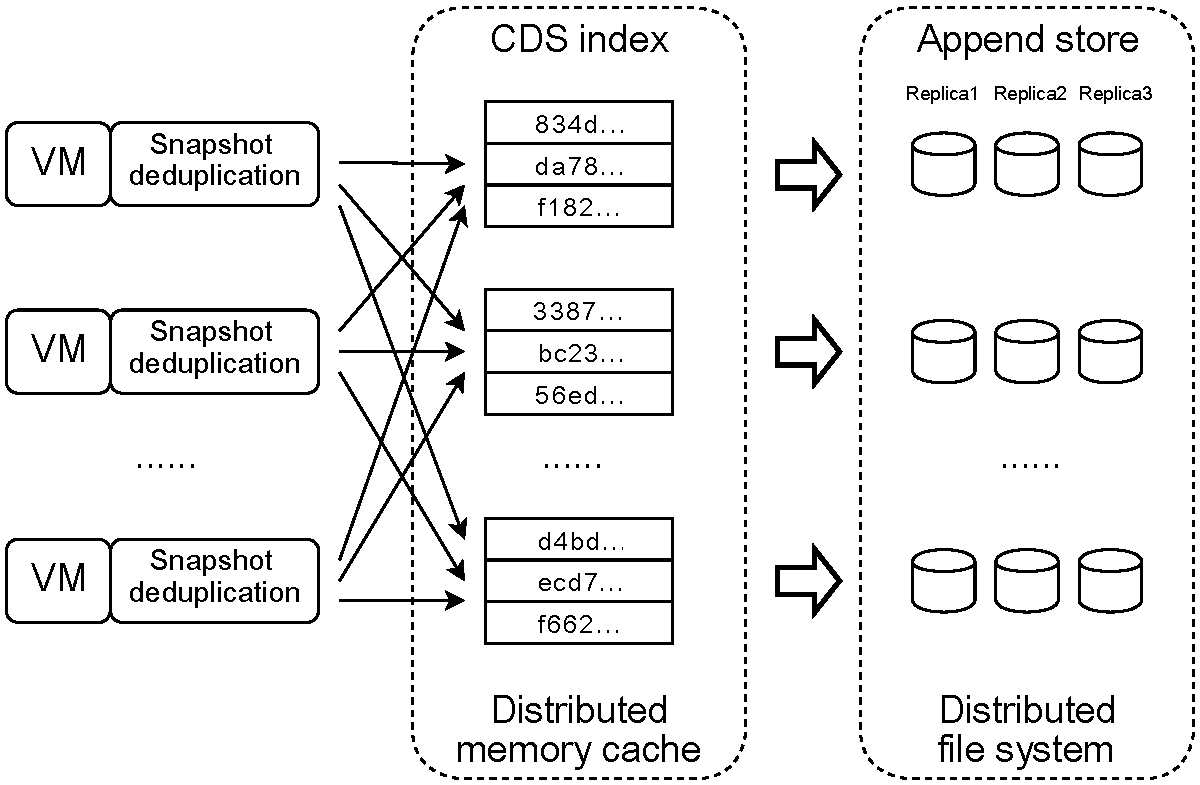
\includegraphics[width=3in]{images/socc_arch_cluster}
        \label{fig:arch_cluster}
    }
    \\
    \subfigure[Node architecture from VM point of view]
    {
        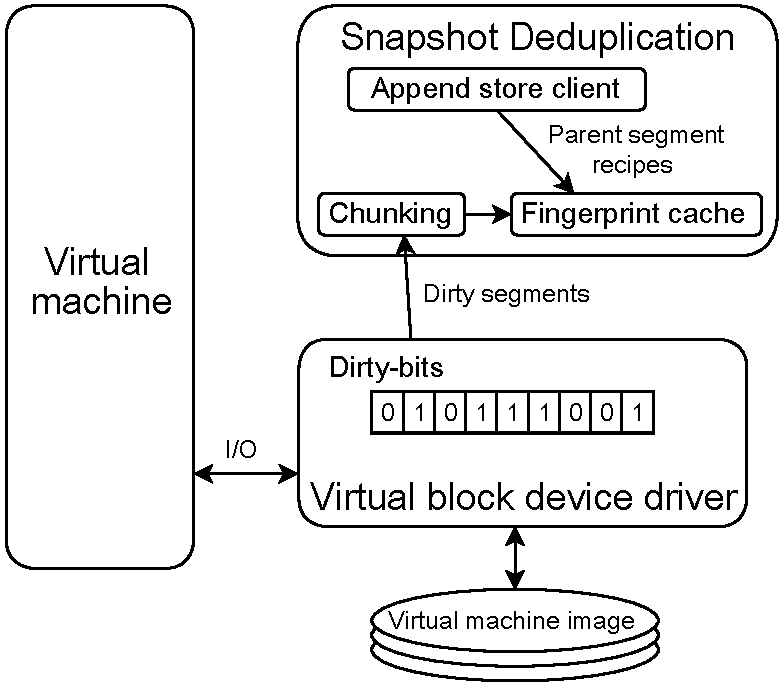
\includegraphics[width=3in]{images/socc_arch_vm}
        \label{fig:arch_vm}
    }
    \caption{System architecture}
    \label{fig:arch}
\end{figure}

\subsection{Architecture}
\label{sect:arch}
%[describe the cloud environment]
Our architecture, as shown in figure.\ref{fig:arch}, is built on top of 
Alibaba's platform which is the largest cloud service provider in China. 

%[describe the arch from cluster side]
{\bf Cluster Architecture}
A typical VM cluster in our cloud environment
consists of from hundreds to thousands of physical machines, each of which can
host tens of Xen-based\cite{Barham2003} VMs.
Alibaba's cloud platform provides a hadoop-like infrastructure, 
which includes several highly scalable distributed service:
\begin{enumerate}
\item {\bf Distributed file system} This is a scalable distributed file system (DFS) being optimized for many large and sequential reads or appends. DFS holds the responsibility of managing physical disk storage
in the cloud. All data needed for VM services, such as virtual disk images used by runtime VMs,
and snapshot data for backup purposes, reside in this distributed file system. 
%\item[KV]: a distributed key-value store for managing structured data.
%\item[MapReduce]: a distributed data processing framework supports Map-Reduce\cite{Dean2004}.
\item {\bf Distributed memory cache} A distributed memory object caching system helps us to hold the fingerprints of those popular data blocks for deduplication inquiries. 
\end{enumerate}
}

\section{Architecture and Implementation Details}
\label{sect:arch}
%[describe what is going to be presented in this section]
%We start by analyzing the main features in the design of our system.
%We first present its architecture,
%then introduce the two major contributions: the colocated deduplication 
%scheme and the snapshot deletion strategy.
%\subsection{Architecture}
%[describe the cloud environment]


%Our architecture, as shown in figure.\ref{fig:arch}, is built on top of 
%Alibaba's platform which is the largest cloud service provider in China. 
%A typical VM cluster in our cloud environment
%consists of from hundreds to thousands of physical machines, each of which can
%host tens of xen-based\cite{Barham2003} VMs.
%Alibaba's cloud platform provides a hadoop-like infrastructure, 
%which includes several highly scalable distributed service:

Our system runs on a cluster of Linux machines with Xen-based VMs.
A distributed file system (DFS) manages  the physical disk storage and we use 
QFS~\cite{QFS}. 
All data needed for VM services, such as virtual disk images used by runtime VMs,
and snapshot data for backup purposes, reside in this distributed file system. 
One physical node hosts tens of VMs, each of which access its virtual machine disk image through the
virtual block device driver (called TapDisk\cite{Warfield2005} in Xen).

\comments{
\begin{description}
\item[Distributed file system] This is a scalable distributed file system (DFS) being optimized for many large and sequential reads or appends. DFS holds the responsibility of managing physical disk storage
in the cloud. 
All data needed for VM services, such as virtual disk images used by runtime VMs,
and snapshot data for backup purposes, reside in this distributed file system. 
%\item[KV]: a distributed key-value store for managing structured data.
%\item[MapReduce]: a distributed data processing framework supports Map-Reduce\cite{Dean2004}.
\item[Distributed memory cache]: A distributed memory object caching system helps us to hold the fingerprints of those popular data blocks for deduplication inquiries. 
\end{description}

In addition, our implementation also uses MapReduce to facilitate the offline
data processing, and stores a small amount of snapshot metadata in a 
BigTable-like persistent key-value store. 

%[describe the benefits of using mature cloud technologies]
In general, our snapshot system and the virtual machine management service 
rely on these fundamental cloud services
to be functional. Such a co-located deduplication architecture allow us 
to enjoy the benefits from these mature technologies 
such as load balancing, scalability, and fault tolerance.
Moreover, all the above cloud services can easily find their open-source counterparts,
which improves the generality of our architecture and deduplication scheme.


%[describe the architecture frm node side]
{\bf Node Architecture} 
Our node-side architecture, depicted in figure.\ref{fig:arch_vm}, consists of
two main entities: a virtual block device driver, and snapshot deduplication component.

%[brief the virtual device driver]
In Alibaba's VM cloud, every VM access its virtual machine disk image through the
virtual block device driver (called TapDisk\cite{Warfield2005} in Xen).
This driver maintains a map of dirty-bits to record
the change status of every fix-size segment of the virtual disk. 
When the VM issue a disk write, the bits corresponding to the segments that covers 
the modified disk region are set, thus letting snapshot deduplication component knows these
segments must be checked during snapshot backup. After the snapshot backup is finished, 
snapshot deduplication component acknowledges the driver to reset the dirty-bits map to
a clean state.

%[brief the snapshot deduplication]
The snapshot deduplication component consists of the chunking and deduplication 
logic of our snapshot storage system. We choose 

It contains an append store client which provides facilities to manage stored snapshot data, and a PDS client to support PDS index access. We will further discuss our deduplication scheme in section\ref{sect:dedupe}.


{\bf Snapshot Representation}
The virtual device driver uses a bitmap to track the changes 
that have been made to virtual disk.
Every bit in the bitmap represents a fix-sized (2MB) region called a \textit{segment}, which indicates whether the segment
has been modified since the last backup. Hence we could treat segment as the basic unit 
in snapshot backup similar to a
file in filesystem backup: a snapshot could share a segment with previous snapshot it has not been changed. 
Moreover, we break segments into variable-sized chunks (average 4KB) using a content-based chunking algorithm,
which brings the opportunity of fine-grained deduplication by
allowing data sharing between segments.
}

\subsection{ Components of a cluster node } 

As  depicted in Figure~\ref{fig:arch_vm}, 
there are four key service components running on each cluster
node  for supporting backup and deduplication: 
1) a virtual block device driver, 2) a snapshot deduplication component,
3) an append store client to store  and access snapshot data,
and 4)  a PDS client to support PDS index access. We will further discuss our deduplication scheme 
in Section~\ref{sect:dedupe}.


We use the virtual device driver in Xen that employs a bitmap to track the changes 
that have been made to virtual disk.
%This driver maintains a map of dirty bits to record the change status of every fix-size segment of the virtual disk. 
When the VM issue a disk write, the bits corresponding to the segments that covers 
the modified disk region are set, thus letting snapshot deduplication component knows these
segments must be checked during snapshot backup. After the snapshot backup is finished, 
snapshot deduplication component acknowledges the driver to reset the dirty-bits map to
a clean state.
Every bit in the bitmap represents a fix-sized (2MB) region called a \textit{segment}, indicates whether the segment
is modified since last backup. Hence we think of segment as the basic unit 
in snapshot backup similar to
file in normal filesystem backup: a snapshot could share a segment with previous snapshot it is not changed. 
As a standard practice, segments are further divided into variable-sized chunks (average 4KB) 
using a content-based chunking algorithm, which brings the opportunity of fine-grained deduplication by
allowing data sharing between segments.

The representation of each snapshot has  a two-level index data structure.
%in the form of a hierarchical directed acyclic graph as shown in Figure \ref{fig:snapshot}.
The snapshot meta data (called snapshot recipe) contains a list of segments, each of which contains segment
metadata of its chunks (called segment recipe).
%\begin{figure}[htbp]
%  \centering
%  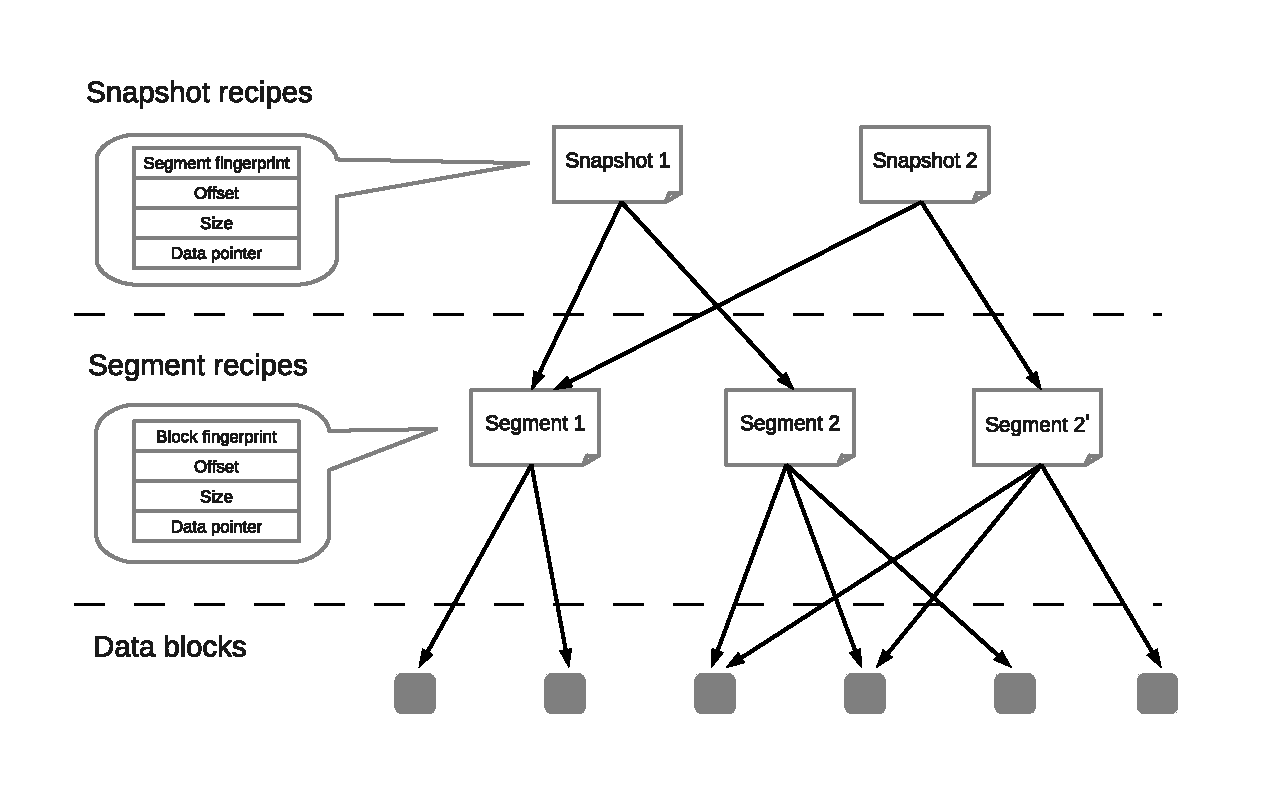
\epsfig{file=images/snapshot_representation, width=3in}
%  \caption{An example of snapshot representation.}
%  \label{fig:snapshot_rep}
%\end{figure}
%As a result, the representation of each snapshot is designed as a two-level index data structure 
%in the form of a hierarchical directed acyclic graph as shown in Figure \ref{fig:snapshot_rep}.
%A snapshot recipe contains a list of segments, each of which is represented as a segment recipe
%that holds the meatdata of its chunks. We choose this two-level structure because in practice we
%observe that during each backup period only a small amount of VM data are added or modified. 
%As the result, even the metadata of two snapshots can be highly similar, 
%thus aggregating a large number of chunks as one segment can significantly reduce the space cost of snapshot metadata.
%Furthermore, instead of using variables-sized segments, we use a dirty bit to capture the change status of fix-sized
%segments which greatly ease the segment-level deduplication.
In snapshot and segment recipes, 
the data structures  includes reference pointers to the actual data location to eliminate the need for additional indirection.
%In our implementation the data reference is a 8 bytes field which is either an 
%ASID (discuss in Section \ref{sect:append}) or an offset of an additional flag indicates
%the location of PDS data.





%\subsection{Snapshot management}


\begin{figure*}[t]
    \centering
    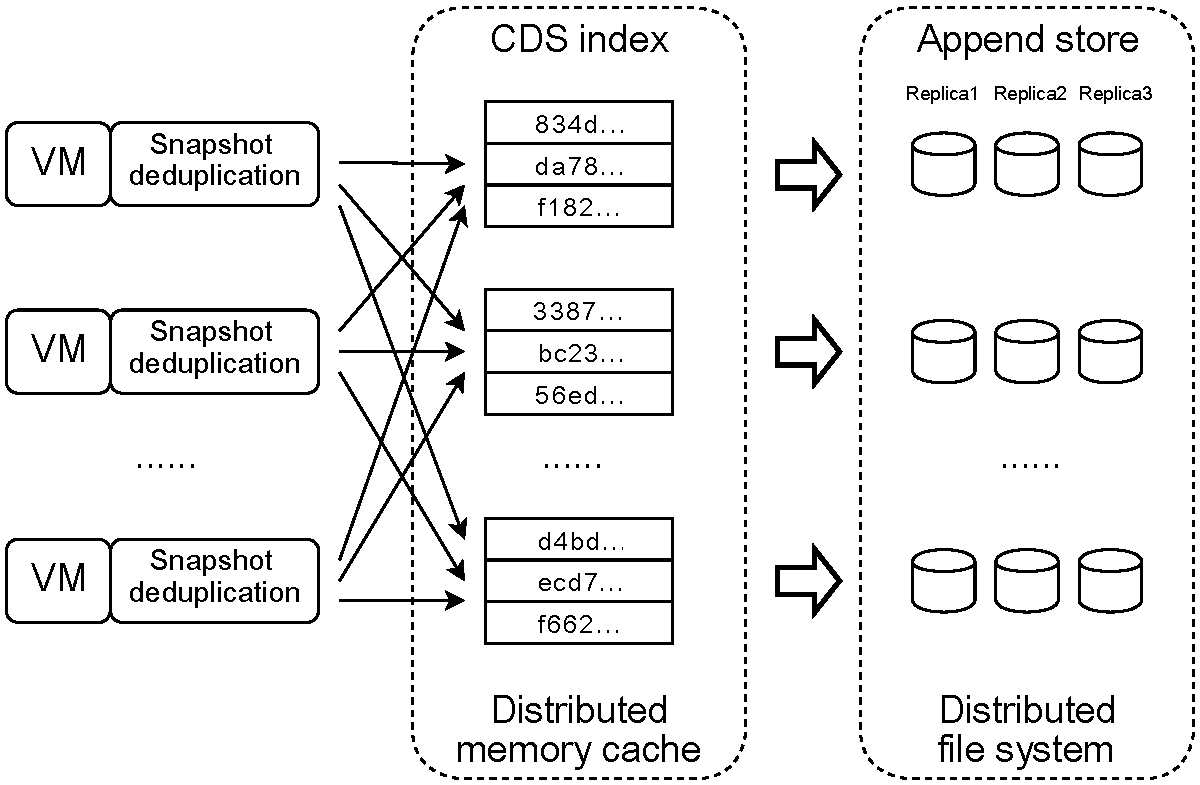
\includegraphics[width=6in]{images/socc_arch_cluster}
    \caption{System Architecture}
    \label{fig:arch_vm}
\end{figure*}

\comments{%socc_arch_cluster now includes the entire arch instead of having 2 figures
\begin{figure}
    \centering
    \subfigure[Node architecture from VM point of view]
    {
        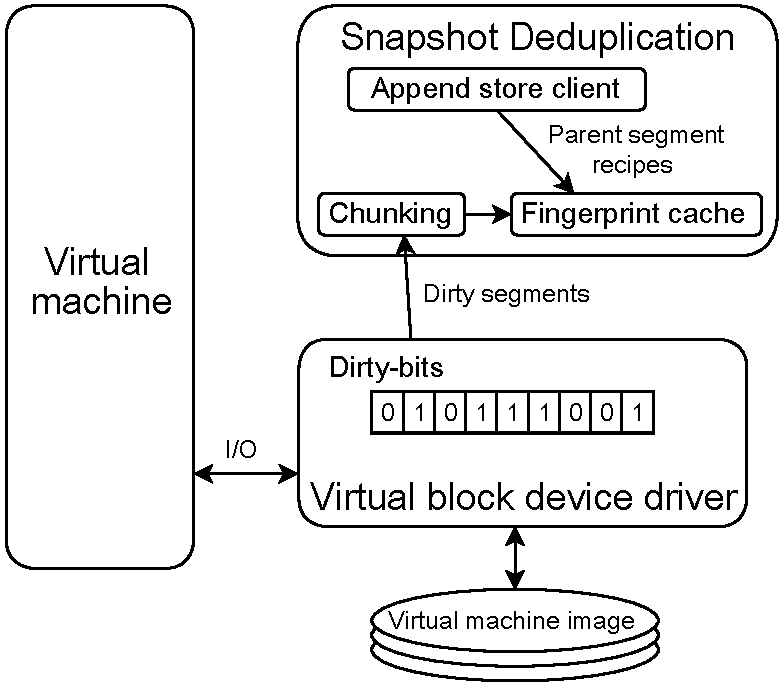
\includegraphics[width=3in]{images/socc_arch_vm}
        \label{fig:arch_vm}
    }
    \\
    \subfigure[Cluster architecture]
    {
        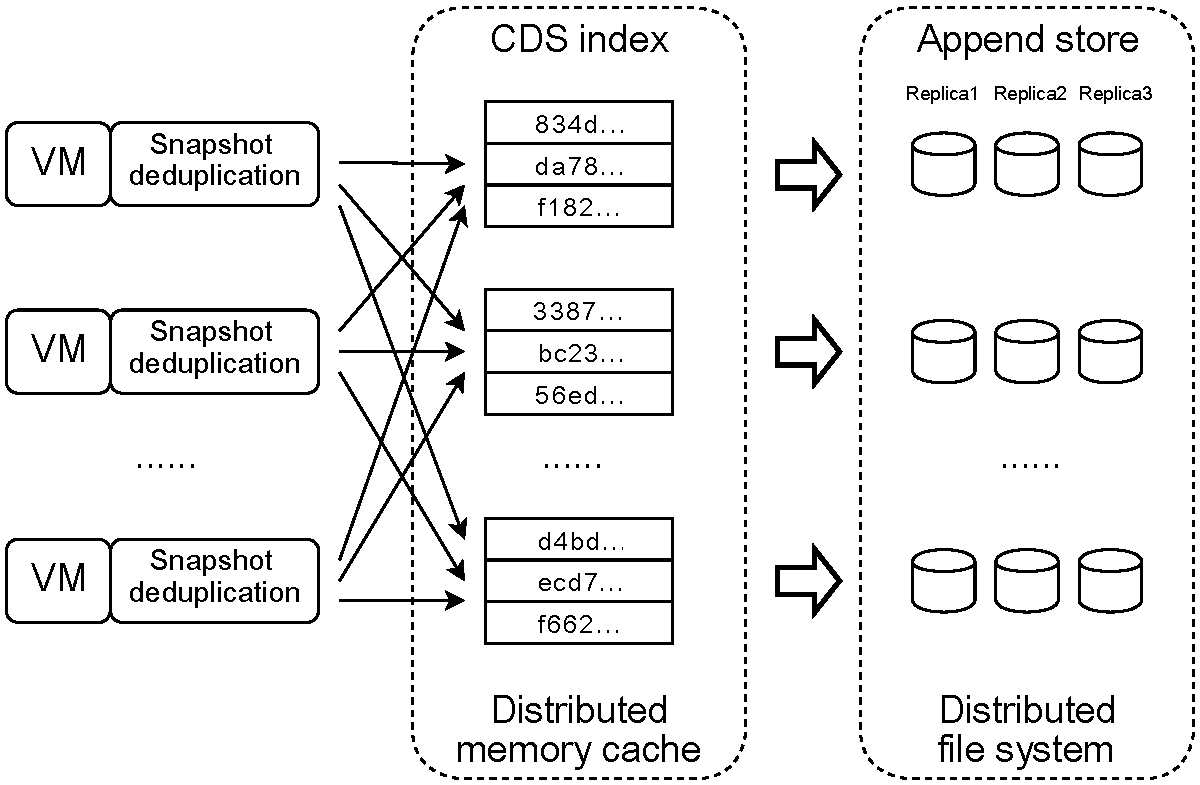
\includegraphics[width=3in]{images/socc_arch_cluster}
        \label{fig:arch_cluster}
    }
    \caption{System architecture.}
    \label{fig:arch}
\end{figure}
}

%[describe the architecture frm node side]
%[brief the virtual device driver]
%One physical node hosts tens of VMs, each of which access its virtual machine disk image through the
%virtual block device driver (called TapDisk\cite{Warfield2005} in Xen).
%This driver maintains a map of dirty-bits to record
%the change status of every fix-size segment of the virtual disk. 
%When the VM issue a disk write, the bits coresponding to the segments that covers 
%the modified disk region are set, thus letting snapshot deduplication component knows these
%segments must be checked during snapshot backup. After the snapshot backup is finished, 
%snapshot deduplication component acknowledges the driver to resume the dirty-bits map to
%a clean state.

%[brief the snapshot deduplication]
%The snapshot deduplication component consists of the chunking and deduplication 
%logic of our snapshot storage system. We choose 

%[describe the arch from cluster side]


%[describe the data structure in underlying storage]
\subsection{A VM-centric snapshot store for backup data}

We build the snapshot storage on the top of a distributed file system.
Following the VM-centric idea for the purpose of fault isolation,
each VM has its own snapshot store, containing new data chunks which are considered
to be non-duplicates.
There is also a special store containing all PDS chunks shared among different VMs.
This separation of PDS chunks allows us to change the replication degree of of those popular file blocks in the underlying file system
Extra replication of this store is added and analyzed in Section~\ref{sect:analysis}.
As shown in Fig.\ref{fig:as_arch}, we explain the data structure of snapshot stores as follows.

\begin{itemize}
\item The PDS snapshot contains a set of commonly used data chunks and is accessed by its offset and size
in the corresponding DFS file.
The PDS index uses the offset and size as a reference in its index structure.
 
\item Each non-PDS snapshot store is divided into a set of containers and each container is approximately 
1GB. The reason we divide the snapshot into containers is to simplify the compaction process
conducted periodically. Chunks without any reference from other snapshots can be removed by this process, and the compaction  routine can work on one container at a time
and copy used data chunks to another container. By limiting the size of a container, we limit the cost of the compaction process.
	\begin{itemize}
	\item Each container is divided into a set of chunk data groups. Each group is composed of
	a set of data chunks and is the basic unit for the snapshot in data access and retrieval. 
	In writing a chunk group, data chunks in this group are compressed together and then stored. 
	When accessing a particular chunk, its chunk group is retrieved from the disk storage
	and uncompressed. Given the high spatial locality 
in snapshot data accessing~\cite{Sampling,FoundationPaper},
	retrieval of  data chunks by group naturally works well with prefetching to speedup
	snapshot access. A  typical chunk group contains 100 to 1000 chunks, with an average size of 
200-600 chunks.
Chunk grouping also reduces the  container index size as we discuss below. 
Given  the average chunk size of 4KB,  the index size for a 1GB container reduces from 10MB to 100KB when
the chunk group size is 100.
%%CBlock, then the overall index size is reduced to $1/m$. 
%n our implementation, using $m=100$ reduces the index for
%a 1GB container from 10 MB to 100 KB.
	\item 
Each data container is represented by three data files in the DFS:
1) the container data file holds the actual content of data chunks, 
2) the container index file is responsible for translating a data reference
into its location within a container, and 
3) a chunk deletion log file saving all the deletion requests within  the container.
A VM snapshot store typically has a small number of containers because each container is fairly large, with an average size of 1GB, and 
maintains a limited number of snapshots (e.g. 10 in the Alibaba case).
New snapshot data chunks can be effectively compressed in chunk groups in addition to  deduplication.

\item We maintain  a chunk counter and assign the current number 
as a chunk ID (called CID) within this container as a reference of a new chunk added to a container. 
Since data chunks are always appended to the snapshot store, 
 a CID is monotonically increasing.
A data chunk reference stored in the index of snapshot recipes
is composed of two parts: a container ID (2 bytes) and CID (6 bytes).
When a snapshot chunk is to be accessed, the recipe for the snapshot will point to either a data chunk
in the PDS or a reference number with a container ID and CID.
With a container ID, the corresponding container index file is accessed and 
the chunk group is identified using this CID. Once the chunk group is loaded to memory, its header contains the exact offset of the corresponding chunk and the content is then accessed from the memory buffer.

%Every container  Store assign every piece of data a CID for its internal data referencing. 
%When new data is appended, its CID is the current largest CID in that container plus one.
%As a result, all the data locations are naturally indexed by this self-incremental CID, 
%no extra sorting is needed.
	\end{itemize}
\end{itemize}

%acceretrieved  and ret
%Using CBlock brings us several advantages: First, the write workload to DFS master is greatly reduced; second, grouping
%small chunks gives better compression. Third, reading a CBlock (200 - 600 KB) typically cost the same amount of disk 
%seek as reading a 4KB chunk. Finally, this greatly reduces the size of index. Let $m$ be the number of chunks in each
%CBlock, then the overall index size is reduced to $1/m$. In our implementation, using $m=100$ reduces the index for
%a 1GB container from 10 MB to 100 KB.

 
% of  divided into a set of data containers.
%Each container has 3 parts.
%Each chunk in the snapshot is referenced by the following data format

%The Append Store (AS) is our underlining storage engine for storing snapshot data in the distributed file system
%after deduplication.
%AS is built on top of our highly scalable distributed file system (DFS), 
%which is very similar to Google's file system
%in a sense that it is optimized for large files and sequential read/append operations.

\begin{figure}[htbp]
  \centering
  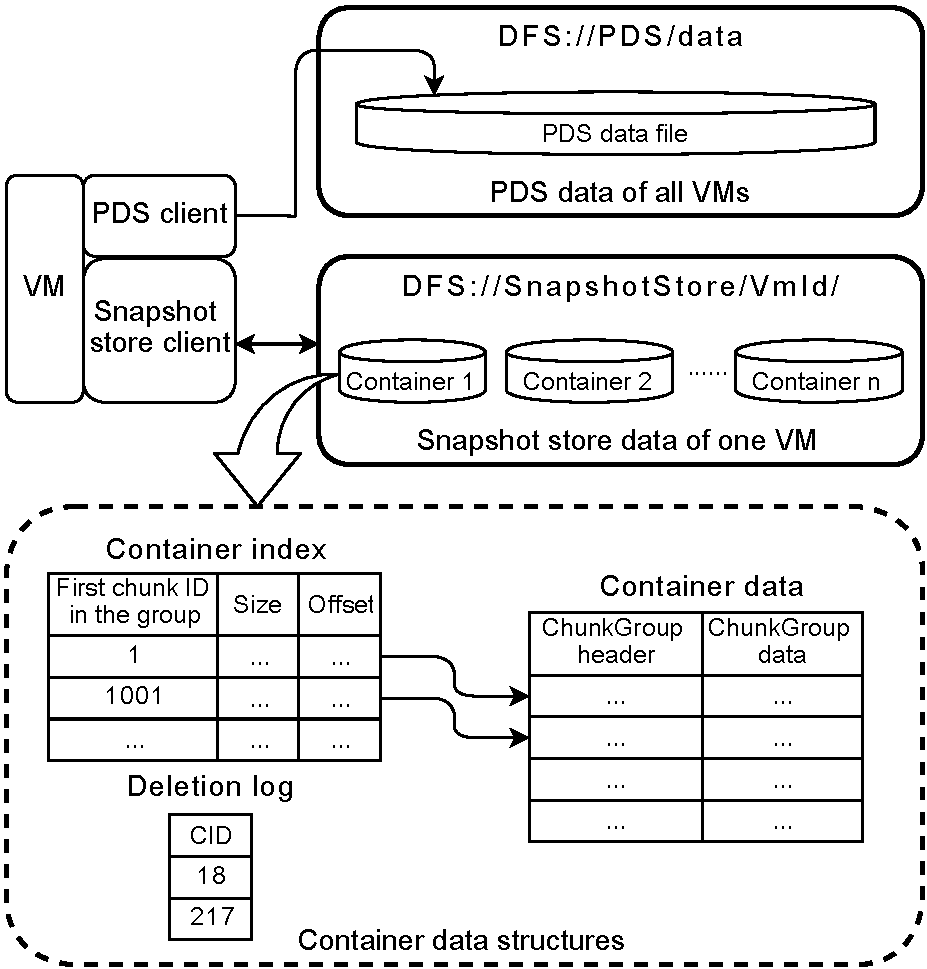
\epsfig{file=images/sstore_arch, width=3in}
  \caption{Data structure of VM snapshot stores.}
  \label{fig:as_arch}
\end{figure}

%\begin{figure}[htbp]
%  \centering
%  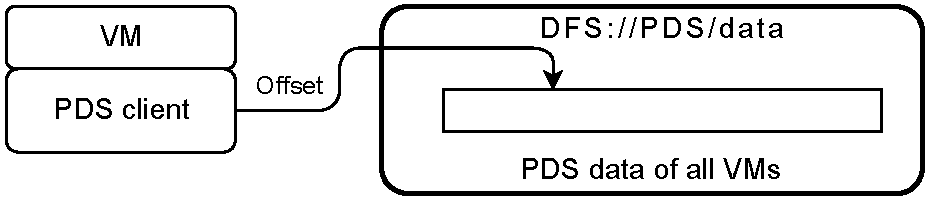
\epsfig{file=images/pds_arch, width=3in}
%  \caption{System architecture for PDS data store.}
%  \label{fig:as_arch}
%\end{figure}

The snapshot  store supports three API calls.
\begin{itemize}

%AS supplies three interfaces: {\em get(ref)} accepts a data reference and retrieves data, 
\item {\em Put(data)} places data chunk into the snapshot store and returns a reference to be stored in 
the recipe metadata of a snapshot. 

The write requests to append data chunks to a VM store are accumulated in the client side. 
When the number of write requests reaches the group size $g$, the snapshot store client compresses
the accumulated   chunk group, adds a chunk group index  to the beginning of the group, and then
appends the header and data  to the corresponding VM file.
A new container  index entry is also created for each chunk group and is written the corresponding
container index file.

The writing of PDS data chunks is conducted periodically when there is a new PDS calculation.
Since the PDS dataset is small, a new PDS file is created during the periodical update.
\item{\em Get(reference)}.
The fetch operation for the PDS data chunk is straightforward since each reference contains 
the offset and size within the PDS  underlying  file.
We also maintain a small data cache for the PDS data service to speedup the process.

To read a non-PDS chunk using a reference,  the snapshot store client first loads the
corresponding VM's container index file specified by the container ID, then searches the chunk
group  that  covers the chunk by the group  CID range.
After that, it reads the whole chunk group from DFS, decompresses it, and seeks to the exact chunk data 
specified by the CID. 
Finally, the client updates its internal chunk data cache with the newly loaded content to 
anticipate future sequential reads.
\item {\em Delete(reference)}.
A data chunk can be deleted when a snapshot expires or gets deleted explicitly by a user.
We will discuss the snapshot deletion in the following subsection.
%deletes the data pointed by the reference.
%Under the hood, small var-sized data are grouped and stored into larger data containers. Each VM has
%its snapshot data stored in its own Append Store, specified by the VM ID. 
%We split every Append Store into multiple data containers so that reclaiming the disk space would not 
%result in rewriting all the data at the same time.
When deletion requests are issued for a specific container,
those requests are simply logged into the  container's deletion log initially and thus  a lazy
deletion strategy is exercised.
Once CIDs appear in
the deletion log, they will not be referenced by any future snapshot and can be safely deleted when needed. 
Periodically, the snapshot  store picks those containers with an excessive
number of deletion requests to  compact and  reclaim the corresponding disk space. 
%The actual compaction will only take place when the number of deleted items 
%reached $d\%$ of container's capacity. 
During compaction, the snapshot store creates a new container (with the same container ID) to replace the 
existing one. This is done by sequentially scanning the old container, copying all the chunks that are not 
found in the deletion log to the new container, and creating new chunk groups and indices. 
Every chunk's CID however is directly copied rather than re-generated. This
process leaves holes in the CID values, but preserves the sorted order.
As a result, all data references stored 
in upper level recipes are permanent and stable, and the data reading process
is as efficient as before. This CID stability also ensures that recipes do not
depend directly on physical storage locations.
\end{itemize}

%As shown in Fig.\ref{fig:as_arch}, every data container is represented as three data files in DFS:
%the data file holds all the actual data, the index file is responsible for translating data reference
%into data locations, and a deletion log file remembers all the deletion requests to the container.
%
%A data reference is composed of two parts: a container ID (2 bytes) and CID (6 bytes).
%Append Store assign every piece of data a CID for its internal data referencing. 
%When new data is appended, its CID is the current largest CID in that container plus one.
%As a result, all the data locations are naturally indexed by this self-incremental CID, 
%no extra sorting is needed.

%Append Store groups multiple chunk data (i.e., 100) into larger units, called {\em CBlock}.
%CBlock is the basic unit for append store's internal read/write/compression.
%There is one index entry in the container index corresponding to every CBlock. It keeps the first chunk's CID
%in that CBlock, and the CBlock data's size and location.
%
%Using CBlock brings us several advantages: First, the write workload to DFS master is greatly reduced; second, grouping
%small chunks gives better compression. Third, reading a CBlock (200 - 600 KB) typically cost the same amount of disk 



\comments{
\subsection{Snapshot Deduplication and Fault Isolation}
\label{sect:dedupe}
%snapshot representation
%\subsection{Inner and corss VM deduplication}
Our  deduplication scheme compares the fingerprints of the current snapshot
with its parent snapshot and also other snapshots in the entire cloud.
This process performs   the duplication in two categories: \textit{Inner-VM} and \textit{Cross-VM}. 
Inner-VM duplication exists between a VM's snapshots, because the majority of data is unchanged during each backup period. 
Such localization decreases data dependencies between different VM backups,
simplifies snapshot management and statistics collection,
and facilitates parallel execution of snapshot operations.
On the other hand, Cross-VM duplication is mainly due to widely-used software and libraries. 
As the result, different VMs tend to backup a large amount of highly similar data.
Our multi-level pipeline process can minimize 
the cost of deduplication while maximize the its efficiency at each level,
and is parallel since each segment is processed independently.

\begin{itemize}
\item \textbf{Dirty-based coarse-grain inner-VM deduplication.}
The first-level deduplication is to follow the standard dirty bit approach, but is conducted
in the coarse grain segment level.
We use the  Xen virtual device driver which supports dirty bits for the storage device
and the dirty bit setting is maintained in a coarse grain level we call it a segment.
In our implementation, the segment size is 2MB. 
Since every write for a block will touch a dirty bit, the device driver maintains dirty bits in memory
and cannot afford a small segment  size.

\item \textbf{Chunk-level fine-grain nearby duplicate detection.}

The best deduplication uses a nonuniform chunk size 
in the average of 4K or 8K~\cite{??}.
Thus the second-level inner-VM deduplication is to assess in this
level, but only for those dirty  segments. 
We load the fingerprints of chunks in the corresponding segment from the
parent for a comparisons and compare near-by fingerprint matching within this segment.
The amount of memory for maintaining those fingerprints  is small.
For example, with a 2MB segment, there are about 500 fingerprints to compare.


%If we use 4KB in level-1, then such a level-1 should have similar dedup efficiency 
%as the current level-1 and level-2 combined, because finally they equal to comparing  
%parent snapshot at 4KB granularity.
%
%However, at level-3 things are different. If we use 4KB fix-size block uniformly, it would be harder for different VM to share data through PDS, because there is no guarantee that the location of duplicate data on different VM disks are always aligned at 4KB boundary. For example, if two VMs each has a copy of duplicate data, but they are not aligned, then we won't be able to detect them. Our study at the current small data set has shown that using 4KB fix-size block will make PDS method less efficient by nearly 10%. Over the long time, more and more OS variations will co-exist in the cluster, making this 4KB fix-size approach inefficient in reducing duplicate data across VMs.

%\item \textit{Level 2  Chunk fingerprint comparison.}
%If a segment is modified, we perform fine-grained deduplication 
%by comparing the fingerprints of its chunks to the same segment's recipe in the previous snapshot,
%thus eliminate partial data duplication within the segment.
%\end{itemize}
%
%In general, operations at level 1 have almost no cost and most of unmodified data are filtered here. 
%To process a dirty segment at level 2, 
%there requires no more than one DFS access to load the segment recipe from previous snapshot,
%and a tiny amount of memory to hold it in main memory.

\item \textbf{Cross-VM deduplication.}
This step accomplishes the standard global fingerprint  comparison as conducted
in the previous work~\cite{??}.
One key observation is that the inner deduplication has removed many of duplicates.
There are not lot of deduplication opportunities cross VMs while the memory
consumption for global comparison is expensive.
Thus our approximation is that duplicate sharing patterns among  VM follows
a zip-like distribution, and the global fingerprint  comparison  only searches
for the most popular items. 
\end{itemize}

{\bf Popular Chunk Management and VM-oriented Fault Isolation}
Our objective for fault isolation is to minimize the number of VMs affected when there are failures
in the cluster.  The inner-VM deduplication does not depend on any global service and the comparison
for each VM is localized within the parent and the current snapshot.
Thus there is no data dependence between VMs.
For cross-VM deduplication, there is a data dependence among VMs and we would minimize the failure impact
of shared blocks by adding extra replicas of those shared blocks.

This section analyzes the choice of popular blocks and its impact on the deduplication efficiency.
It also  compares the  fault resilience of our VM-centric deduplication approach with a standard approach using 
global deduplication.


{\bf Impact of PDS deduplication.}
Our empirical study based on VM images from production environment\cite{ieeecloud} showed that the
frequency of data duplication follows Zipf-like distribution\cite{zipf},
with the exponent $\alpha$ between 0.65 ~ 0.70.
As a result, it can be proved that deduplication efficiency of PDS index is scalable:

For the Zipf-like distribution, an approximation to the sum of the first $n$ 
elements of the distribution can be derived as follows:
\begin{equation}
\sum_{i=1}^{n}\frac{1}{i^\alpha}\approx \int_{1}^{n}\frac{1}{x^\alpha}\mathrm{d}x=\frac{x^{1-\alpha}}{1-\alpha}=\frac{n^{1-\alpha}}{1-\alpha}\;  for\;  \alpha<1
\end{equation}
So the cumulative distribution function for a PDS holding top $S_c$ fingerprints
of global index with size $S_g$ is:
\begin{equation}
  E = (S_c / S_g)^{1-\alpha} \;  for\;  \alpha<1
\end{equation}
%[Describe the dedup efficiency model in detail]
Let $N$ be the number of nodes in the cluster, $m$ be the memory on each node that are used by PDS, $D$ be the amount of data on each node, and $B$ be the average block size. Then $S_c$ and $S_g$ can be expressed as:
\begin{equation}
S_c = N*m/F, \; S_g = N*D/B
\end{equation}
By replacing $S_c$ and $S_g$ in the first formula, the deduplication efficiency becomes:
\begin{equation}
  E = (\frac{m*B}{F*D})^{1-\alpha}
\end{equation}
Since $B$, $D$ and $F$ are pre-configured constants, the deduplication efficiency of PDS is only controlled by the its memory usage.

\begin{table}
    \begin{tabular}{llll}
    Data size (GB) & 1\%    & 2\%    & 4\%    \\
    14.6           & 18.6\% & 22.1\% & 31.4\% \\
    28.1           & 19.5\% & 26.2\% & 38.8\% \\
    44.2           & 21.7\% & 26.5\% & 36\%   \\
    61.6           & 23.2\% & 32.9\% & 35\%   \\
    74.2           & 23.6\% & 33.6\% & 37.5\% \\
    \end{tabular}
    \caption{Deduplication effectiveness of top k\% of global index}
    \label{tab:cds}
\end{table}

}

\subsection{ VM-centric Approximate Snapshot Deletion with Leak Repair}

\begin{figure}[htbp]
  \centering
  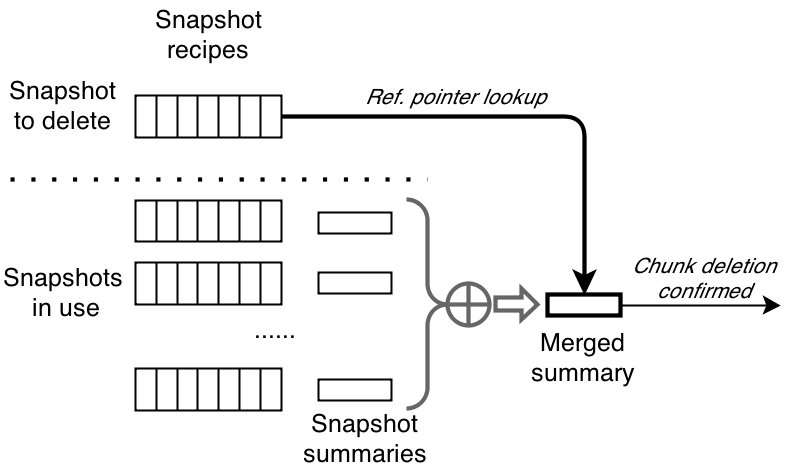
\epsfig{file=images/deletion.png, width=3.5in}
  \caption{Approximate deletion}
  \label{fig:deletion_flow}
\end{figure}

In a busy VM cluster, snapshot deletions are as frequent as snapshot creations.
However, data deduplication complicates the deletion process because space saving relies on the sharing of data,
thus making it difficult to decide which chunks are safe to delete.
In a traditional deduplication system, deletion often require looking at global scope to
resolve the data dependency between logical backup entities and physical data chunks.
Our VM-centric snapshot storage design simplifies the deletion process since 
we only need to locate unreferenced chunks within each VM's snapshot store to free up space when deleting a snapshot.
The PDS data chunks are commonly shared all VMs and we do not consider their reference
counting during snapshot deletion.
%The selection of PDS data chunks is updated periodically independent of snapshot deletion process.

While we can use the standard mark-and-sweep technique~\cite{mark-sweep}, 
it still takes significant time to conduct this process every time there is a snapshot deletion.
In the case of Alibaba, snapshot backup is conducted automatically and there are 
about 10 snapshot stored for every user. When there is
a new snapshot created every day,  there will be  a snapshot expired everyday to maintain
a balanced storage use. Given the large number of snapshot deletion requests, we seek
a fast solution with a very low resource usage to delete snapshots.

With this in mind, we develop an {\em approximate} deletion strategy to trade deletion accuracy for
speed and resource usage. Our method sacrifices a small percent of storage leakage
to effectively identify unused chunks in $O(n)$ time, with $n$ being the logical number of non-PDS chunks 
to be deleted from a VM snapshot store.
The algorithm contains three aspects.


%Our system adopts VM-centric snapshot  lazy delete strategy so that all snapshot deletions are scheduled
%in the backup time window at midnight. 
%Therefore, snapshot deletions must be fast enough to fit in time window and
%efficient enough to satisfy our resource constraints.
%However, there is no simple solution can achieve these goals with high reliability.
%Our hybrid deletion strategy, using fuzzy deletion regularly and accurate deletion periodically,
%accomplishs our speed, resource usage and relibility goals very well.
\begin{itemize}
\item {\bf Computation for snapshot fingerprint summary.}
Every time there is a new snapshot created,
we compute a bloom-filter with $z$ bits as the summary of reference pointers for all non-PDS chunks used 
in this snapshot. 

%To control the false positive ratio $\epislon$ under $0.01$, an average snapshot of size 40 $GB$ with 
%$u \approx 10$ million chunks, $z$ has 10 million bits. 

%{\bf Creating bloom filter} Scan all the living snapshot recipess and their segment recipes,
%for every reference pointing to append store, add it to the bloom filter.

\item {\bf Approximate deletion with fast summary comparison.}
Then when there is a snapshot deletion,  
we need to identify if  chunks to be deleted from one snapshot
are still used by other snapshots. 
This is done approximately and quickly by comparing the reference pointers of deleted snapshots with
the merged reference bloom-filter summary of other live snapshots.
The merging of live snapshot bloom-filter bits uses the logical OR operator and the merged vector still takes $z$ bits.
Since the number of live snapshots is limited for each VM (e.g. 10 in the Alibaba's production system), 
the time cost of this comparison is small.
%Instead of scanning the entire append store indices, we merge the type-1 summaries of all
%valid snapshots. 
%Since each VM has uniform bloom filter parameters to create snapshot summaries, 
%such merged summeries give us a compact representation of
%all block fingerprints that are still in use.
%Thus by the property of bloom filter, if a fingerprint is not found in merged summaries, 
%we are certain that block is no longer used by any valid snapshot, it would be then added
%to append store's deletion log.
However, there is a small false-positive ratio which
would identify unused data as in use, resulting in temporary storage leakage.


\item {\bf Periodic repair of leakage}
%[exlpain why second bloom filter, why scan append store]
Since there are certain unused chunks which are not deleted during
the approximate deletion, leakage repair is conducted periodically.
In this phase we load the reference pointers of all chunks from a VM snapshot store as a table in memory,
then scan through all the snapshots' segment recipes. For each reference pointer that is in use by a snapshot,
we mark the corresponding entry in the table as in use. Finally those unmarked (and therefore unused) reference pointers in the
table represent chunks that can be safely deleted.

The cost of leak repair mainly come from holding a table of reference pointers and the scan of all snapshots' metadata.
Consider each reference pointer consumes 8 bytes plus 1 byte as mark field, a VM that has 40GB backup data with about
10 million chunks will need 90MB of memory to construct such a table. 
Also, scanning all snapshots metadata is many times slower when compared
to the approximate deletion which only scans single snapshot's metadata.
It's worth mention that compared to previously-developed mark-and-sweep techniques, 
our leak repair still has advantages because the scope of repair is restricted within a single VM's snapshot 
store due to our VM-centric design, and we perform leakage repair periodically.
%We cannot simply repeat the phase 1 multiple times to reduce temporary storage leakage, because:
%\begin{enumerate} 
%\item After several runs of phase-1, it is proven that the merged type-1 summaries cannot sieve remaining unused blocks, due to the false-positive property of bloom filter.
%\item The recipes of deleted snapshots have been removed from the system, thus we are not able to obtain the deleted block fingerprints from any metadata, the only way to discover them is to scan the append store indices.
%\end{enumerate}
\end{itemize}




%\item {\bf Check existance} For every data reference in the deleted snapshot recipe and its segment recipes,
%check the existance of that data reference in bloom filter. If not found, it is safe to delete that piece of data from append store
%because no living snapshots has referenced it.

%The overall time of running a approximate deletion for one snapshot deletion would be scanning
%all the living snapshots and deleted snapshots, since operations on the in-memory bloom filter can be done in
%parallel and is much faster than loading recipes from DFS:
%\begin{equation}
%T = (N_{SS} + 1) * T_{scan\_recipes}
%\end{equation}
%
%Using the example and analysis in previous section, this approximate deletion can be done in 5 minutes.
%Memory usage of the bloom filter depends on its false-positive probility $P_{bl}$,
%when set $P_{bl}$ to 0.01, the memory footprint of approximate deletion is about 15 MB.
%~



%{\bf Discussion}
We now estimate the storage leakage and how often leak repair needs to be conducted.
Assuming a VM always maintain $h$ snapshots in the backup, and it creates and deletes one snapshot
everyday. Let $u$ be the total number of chunks brought by the initial backup, $\Delta u$ be the average
number of additional unique chunks added from one snapshot to the next snapshot. Then the total number of unique
chunks used is about:
\[
U = u + (h-1)\Delta u.
\]

Each bloom filter vector has  $z$ bits for each snapshot and let $j$ be the number of hash functions used by the
bloom filter. The probablity that a particular bit is still in all $h$ summary vectors is still 0 is 
$(1- \frac{1}{z}) ^{j U}$. Notice that when a chunk appears multiple times in these summary vectors, it does not 
increase the probability of a particular bit being 0 in all $h$ vectors.
Then the false-positive rate $\epsilon$ is: 
\[
\epsilon = (1-(1-\frac{1}{z})^{jU})^j.
\]

For each snapshot deletion, the amount of chunks need to be deleted is nearly identical to the number of
newly add chunks $\Delta u$. However, some of chunks among them are not detected as unused in our approximation
algorithm, thus forms the storage leakage. Let $R$ be the total number of runs of approximate deletion since
last repair. we estimate  the total leakage $L$ after $R$ runs as:
\[
L = R \Delta u \epsilon
\]

When leakage ratio $L/U$ exceeds a pre-defined threshold $\tau$, we need to execute a leak repair:
\[
\frac{L}{U} = \frac{R \Delta u \epsilon}{u+(h-1)\Delta u } > \tau 
\Longrightarrow R > \frac{\tau}{\epsilon}\frac{u + (h-1)\Delta u}{\Delta u}
\]
For example in our tested dataset,  
each VM keeps $h=10$ snapshots and each snapshot has
about 1-5\% of new data. Thus $\frac{\Delta u}{u}=0.05$ at most. With 40GB snapshot size, $u\approx = 10$ millions.
Then $U=10.45$ millions.
We choose  $\epsilon = 0.01$ and $\tau=0.1$. Then from the bloom filter  false positive formula, 
$z=10U=100.45$ million bits. $R=290$.
Then we would expect leak repair be triggered once for 
every 290 runs of approximate deletion. 
When one machine hosts 25 VMs and there is one snapshot deletion per day per VM, there would be 
only one full leak repair for one VM scheduled for every 12 days. Each repairs uses about 90MB memory on average
as discussed earlier and takes a short period of time.
% which is sufficiently small to offset the heavy I/O workload of the mark-sweep process.
 %, design considerations, architecture
%\comments{
\section{ Old Performance Analysis and Comparison}
\label{sect:analysis-old}

We assume a flat architecture that we use all machines in a cluster to host virtual machines, and also evenly host  raw data and meta data of the temporarily accumulated requests.  We call global index to be the meta data of all non-duplicate chunks such as chunk fingerprints and reference pointers.

Following parameters are used to analyze the performance of our system.
\begin{itemize}
\item
$p$ is the number of machines in a cluster. These machines can run in parallel for backup. The request buckets are evenly distributed among these machines.
\item $v$ is the number of virtual machines per machine. At Alibaba, $v=25$.
\item $x$ is the number of snapshots saved for each VM.
\item $k$ is the number of iterations to complete all virtual machine backup. Each iteration performs v/k backups.
\item $t$  is the  amount of temporary disk space used per physical machine for deduplication.
\item $m$ is the amount of memory used per each physical machine for deduplication. Our goal is to minimize 
\item $s$ is the average size of virtual machine image. At Alibaba data we have tested, $s=40GB$.
\item $d_1$  is the average  deduplication ratio using  segment-based dirtbit.  s*d1 represents the amount of data items that are duplicates and can be avoided for backup. For Alabalba dataset tested, 
$d_1$=77\%.
\item $d_2$ is the average  deduplication ratio using content chunk fingerprints after segment-based deduplication. For Alaba dataset tested,  $d_2=50$\%.
\item $b$ is the average disk bandwidth for reading from local storage at each machine. 
\item $q$ is the number of buckets to accumulate requests at each machine. Thus the total number of buckets is $p*q$.
\item $c$ is the chunk block size in bytes.  In practice $c=4KB$.
\item $u$ is the record size of detection request per block.  In practice, 
\item $u$=40. That includes block ID and fingerprint.
\item $m$ is the maximum memory allocated for deduplication purpose.  A $g$ fraction used for 
machine-machine network  request buffering and $(1-g)$ fraction used for memory-disk bucket buffering.
\item $e$ is the size of a duplicate summary record for each chunk block.
\item $\alpha_n$ is the startup cost for sending a message in a cluster. $\alpha_d$ is the startup cost 
such as seek for disk IO. $\beta$ is the time cost for in-memory duplicate comparison.
\end{itemize}
The system keeps at most  $ x$ copies of snapshots for each VM on average.  The total size of  global content fingerprints is $x*s*v/c*u *(1-d1)*(1-d2)$ where $c$ is the average chunk size and $u$ is the meta data size of each chunk fingerprint. In practice $c=4K$ and $u/c$  is about 100.  $x=10$ in the case of Alibaba cloud.

Define $r = s v (1-d_1)/(ck)$  which is the total number of duplicate detection requests issued at each machine and at each iteration.

We first discuss the memory usage and processing time  of 3 steps. 
 For Step 1,  the buffer for sending requests from one machine to another has a size of  $g*m/p$, and with such a buffering, the total number of outgoing communication messages from  each machine to other machines  can be 
\[
r u p/(g*m)
\]
The total  amount of data communicated among machines is relatively small: $r u p$ in the cluster, distributed among $p$ machines.

Once every machine receives detection requests and divide them into buckets, it writes the content to the disk once the buffer is full. The buffer for each bucket is $(1-g)m/q$ and the total number of disk write requests issued after the bucket buffer is full is:
\[
r u q/((1-g)*m)
\]
The total time for step 1  which  reads VM images and write accumulated detection requests  is:   
\[
r  ( c+  u) /b   +r u /m (\alpha_n  p/g  + \alpha_d q/(1-g)  )
\].

For Step 2,  part of memory at each machine is  to hold  a bucket of global index and accumulated requests. That is
\[
m_b= x*r *u*k(1-d_2)/q + r*u/q
\]
Thus the memory requirement for this portion can be made very small when setting a large q. On the other hand, as the system detects duplicates per hash bucket, we need to allocate buffer space for receiving  duplicate summary for each VM.  The total buffer size is $m-m_b$ which is used evenly for $v$ VMs.

The size of  the duplicate summary for each bucket is
\[
S_{sum}= sv(1-d_1)e /(k c q)
\]
We can buffer the outcome of multiple buckets. The total buffer factor is 
\[
(m-m_b)/ S_{sum}.
\]
The final bucket buffer for each VM is still fairly small, and writing such a buffer to the disk may involve two I/O requests (one to fetch the old block, and one is to update). The total seek cost involved 
\[
2*v*\alpha_d*q/ ((m-m_b)/S_{sum})= 2v r e  \alpha_d / (m-m_b)
\]
Thus the total time of Step 2 takes
\[
( x*r *k*u*(1-d_2) + r*u) / b_d  + r* \beta+   2v *r*e \alpha_d /  (m-m_b).
\]


The key cost of step 3  is to read the nonduplicate parts of each VM and output the backend storage. The time of Step 3  takes:
\[
2 r *c* (1-d_2) /b_d
\]
That assumes that when a content chunk is not a duplicate, there is a significant number of non-duplicate  chunks following that  chunk. 

Thus the total time to process all $v$ virtual machines after $k$ iterations are:
\[
k [
r  ( c+  u) /b   +r u /m (\alpha_n  p/g  + \alpha_d q/(1-g)  )
\]
\[
+( x*r *k*u*(1-d_2) + r*u) / b_d  + r* \beta+   
\]
\[
2v *r*e \alpha_d /  (m-m_b)
+2 r *c* (1-d_2) /b_d
]
\]
subject to conditions that
\[
m - m_b> 0
\]

The total disk requirement  per machine for hosting the global index  and meta  data of  accumulated requests is:
\[
x*r *k*u*(1-d2) + r*u.
\]
That is not so big, and is acceptable as we show later.
}



\section{Performance Analysis and Comparison}
\label{sect:analysis}

\begin{table}[ht]
\centering
\begin{tabular}{|p{0.50cm}|p{7cm}|}
\hline
$p$ &  the number of machines in the cluster\\ 
\hline
$v$ & the number of VMs per machine. At Alibaba, $v=25$\\
\hline
$x$ & is the number of snapshots saved for each VM. At Alibaba, $x=10$\\
\hline
%$k$ & the number of iterations to complete all virtual machine backup. Each iteration performs v/k backups.\\
%\hline
$t$ & the amount of temporary disk space used per machine for deduplication\\
\hline
$m$ & the amount of memory used per machine for deduplication. Our goal is to minimize this\\
\hline
$s$ & the average size of virtual machine image. At Alibaba, from our collected data, $s=40GB$\\
\hline
$d_1$ & the average  deduplication ratio using segment-based dirty-bit. $d_1=77\%$\\
\hline
$d_2$ & the average  deduplication ratio using content chunk fingerprints after segment-based deduplication. For Alaba dataset tested,  $d_2=50$\%\\
\hline
$d_3$ & the average number of dup-with-new blocks, as a fraction of $r$ (defined below)\\
\hline
$b_r$ & the average disk bandwidth for reading from local storage at each machine\\
\hline
$b_w$ & the average disk bandwidth for writing to local storage at each machine\\
\hline
$b_b$ & average write bandwidth to back-end storage (block store)\\
\hline
$q$ & the number of buckets to accumulate requests at each machine. (total number of buckets is $p*q$)\\
\hline
$c$ & the chunk block size in bytes.  In practice $c=4KB$\\
\hline
$u$ & the record size of detection request per block.  In practice, $u$=40. That includes block ID and fingerprint\\
\hline
$e$ & the size of a duplicate summary record for each chunk block\\
\hline
$m_n$ & the memory allocated to network send \& receive buffering. Total network memory is $2m_n$, wich each buffer of size $m_n/p$\\
\hline
%$m$ & the maximum memory allocated for deduplication purpose.  A $g$ fraction used for machine-machine network  request buffering and $(1-g)$ fraction used for memory-disk bucket buffering\\
%\hline
$\alpha_n$ & the latency for sending a message in a cluster\\
\hline
%$\alpha_d$ disk latency\\
%\hline
$\beta$ & time cost for in-memory duplicate comparison\\
\hline
\end{tabular}
\caption{Modeling  parameters and symbols.}
\label{tab:symbol}
\end{table}

Here we develop a model for the total backup time, which becomes important in
trying to minimize the CoW cost during backup \emph{CoW should be explained and
justified before this point in the paper}.  The backup process can be broken
into 4 stages, where the first 3 stages each have two parts, first an
all-to-all exchange of
data, then local processing to prepare for the next stage.

The system keeps at most  $ x$ copies of snapshots for each VM on average.  The
total size of  global content fingerprints is $x*s*v/c*u *(1-d1)*(1-d2)$ where
$c$ is the average chunk size and $u$ is the meta data size of each chunk
fingerprint. In practice $c=4K$ and $u/c$  is about 100.  $x=10$ in the case of
Alibaba cloud.

Define $r = s v (1-d_1)/c$  which is the average number of detection
requests made by each machine, and the number of detection requests each
machine must handle.  We assume the load, i.e., amount of data to backup at
each machine, is not balanced, so there is also $r_max$, which is the number of
requests at the most heavily loaded machine. This is the case in the Alibaba
cluster, with some machines being terabytes while the average machine is 40GB.

In Stage 1a, the dirty segments are read from the virtual disk, the hash of
each block is computed, and dedup requests are sent to the machine hosting the
blocks' respective partitions. Due to the synchronization in each stage, Stage
1a needs to wait for the most heavily loaded machine to read all it's data - so
the read stage depends on $r_{max}$, while the write stage, which is balanced
by the hash partitioning, depends on $r$. We first read $r$ blocks from disk,
send $r$ dedup requests, and then save the received requests to temporary files
(one for each parition). The time for the first stage can be expressed as:
\[
    r_{max} c / b_r + \alpha_n\frac{u r_{max}}{m_n} + r u / b_w
\]

In Stage 1b, each partition index is read from disk, then the dedup requests
(from Stage 1a) for that paritition are processed and the dedup results are
written
back out to disk. The results are broken into 3 groups for each partition:
duplicate blocks, new
blocks, and dup-with-new blocks, which are duplicates of blocks that are new to
this batch.

Let $n$ be the total number of index entries at each machine before the backup
was started.  $n=(v x)(1-d_1)(1-d_2)\frac{e}{c}$. Since each machine holds a
constant number $q$ paritions, and the paritions are uniform in size as they
are from the hash of the block, $n$ is very even across the machines, even when
the vm load is imbalanced.

The cost of Stage 1b is:
\[
    r u / b_r + n e / b_r + r \beta + r e / b_w
\]

In Stage 2a the new block results from Stage 1 are sent to the requesters, and
in Stage 2b the new blocks are written out to the storage system. We will now
mostly be dealing with the $r(1-d_2)$ blocks that are new to the system (or
$r_{max}(1-d_2)$ when we must wait for the most heavily loaded machine). In 2b
the dedup new block results must be read and the actual disk blocks for each
new block
must be re-read before they can be sent to the block store. To avoid seeking
we have found it faster to simply re-read all the dirty data and ignore the
duplicate blocks rather than find only the new blocks on disk. The CoW locking
on the filesystem cannot end until after the dirty data is re-read in Stage 2b.

The cost of Stage 2a is:
\[
    r(1-d_2)e / b_r + \alpha_n\frac{e r_{max}(1-d2)}{m_n} + r_{max}(1-d_2)e / b_w
\]
and the cost of Stage 2b is:
\[
    r_{max}c / b_r + r_{max}(1-d_2)e / b_r% + r_{max}(1-d_2)c / b_b
\]

After the new blocks have been written to the block store, and references to
them have been obtained, those references must be returned to the parition
index holder so that those blocks may be deduped in the future (and also so
dup-with-new requests can be handled in this round). This Stage 3a, to read the
new index entries, return them to the parition index holder, and save the
received references, costs:
\[
    r_{max} (1-d_2)e / b_r + \alpha_n\frac{e r_{max}(1-d_2)}{m_n} + r(1-d_2)e / b_w
\]

Stage 3b consists of updating the partition index with the new block references
from Stage 3a, and also updating the dup-with-new results from Stage 1. First
we load the new references from Stage 2b into memory, and then dedup the
dup-with-new requests against the new block references. Once the dup-with-new
results have chunk references, we can add the dup-with-new results to the
duplicate result files initially created in 1b. We then add the new references
to the corresponding
partition indices to handle future dedup requests. Stage 3b costs:
\[
    r ((1-d_2) + d_3)e/b_r + r d_3\beta + r((1-d_2) + d_3)e / b_w
\]

In the final stage (Stage 4), all duplicate references (including the
dup-with-new references from 3b) are returned to the requesters, so that the
snapshot recipes may be updated with references to those blocks. This process
costs:
\[
    r d_2 e / b_r + \alpha_n\frac{e r_{max} d_2}{m_n} + r e / b_w
\]

%Memory Requirments:\\
%In every stage we need 1 disk read buffer, And then additionally we need the following:
%\begin{description}
%    \item[Stage 1a] network buffers, and $q$ disk write buffers
%    \item[Stage 1b] $n/q$ partition index space, and $p$ disk write buffers (for dedup responses)
%    \item[Stage 2a] network buffers, $v$ disk write buffers (for dedup responses)
%    \item[Stage 2b] 1 disk write buffer (to write out new blocks)
%    \item[Stage 3a] network buffers, $q$ disk write buffers (to write out new refs)
%    \item[Stage 3b] 1 disk write buffer (to update patition index with new blocks)
%    \item[Stage 4] network buffers, $v$ disk write buffers
%\end{description}




\subsection{A Comparison with Other Approaches}
\comments{
The memory  space requirement for the data domain approach with bloom filter is:
\[
x*r k u (1-d2)/r
\]
where $r$ is the bloom filter with about  1:10 ratio in practice.  The disk space used  is 
\[
x*r *k *u*(1-d_2).
\]
}

 %, design considerations, architecture
\section{Round Scheduling}
\label{sect:scheduling}
The simplest way to take advantage of the efficiency of batch processing is to
schedule all the work to be done in one round.  This works well if all of the
data being backed up is just copies (e.g. a separate backup system which data
is sent to over the network), however in our case we are backing up the
original virtual disk, which may still be in use during the snapshot. This adds
extra complexity to the cost analysis, because we must now also consider the
cost of maintaining a constistent view during the snapshot process. We use the
Copy on Write (CoW) provided by the virtual disk manager. With CoW, the
duration of the backup affects how much data must be copied. Other studies have
shown that as much as 8\% or even more of total capacity must be reserved for
CoW \cite{EMCIncrementalDataChanges}. The actual cost of CoW is a factor of the
data size, the write rate, and duration CoW is taking place. The data size
isn't something we can change, nor the write rate, but we can minimize the
duration that a given VM is undergoing CoW. We assume a poisson distribution of
writes (which closely fits the meaured results from
\cite{EMCIncrementalDataChanges}), and then try to minimize the CoW cost using
our performance and CoW model. Although the single batch schedule completes the
backup in the smallest amount of time, it also has the greatest CoW cost
because the most processing must be done before any VM can release the CoW
lock.

Our basic CoW cost model is:
\[
    CoW=n(1-e^{-m/n})
\]
    where \[ m=tw(1-d_1)c \]
$n$ is the number of dirty segments, $t$ is the time under CoW, $w$ is the
write rate during CoW, $d_1$ is the \% of clean data (which doesn't go under
CoW), and $c$ is a constant determining how likely writes are to touch dirty
segments which haven't yet been copied vs. dirty segments which have already
been copied during the current backup. With this CoW cost model and the earlier
performance model, we can estimate the CoW cost of a given backup schedule.
Note that CoW ends in Stage 2b, so only the time up to the end of 2b counts
towards CoW. \todo{we still need to pick a value for $c$}

The way to decrease the CoW cost is to break up the backup into multiple
rounds, where in each round the CoW cost is minimized. The more rounds there
are the shorter each round can be and therefore the smaller the CoW cost. The
more rounds there are however the greater the backup overheads and some of the
efficiency gained from batch processing is lessened. We balance these costs by
setting a time limit on the whole backup job, and then develop an algorithm to
schedule VMs into rounds.

With these goals a model that closely fits our goals is the dual version of the
bin packing problem. In standard bin packing the goal is to fit all of the
items into as few bins as possible, without overfilling any bins. In the dual
version of the problem however as many bins as possible are to filled to at
least some minimum level. In our problem the constraint is to keep the total
cost of the schedule under a time limit rather than a minimum bin level. We
adapt an algorithm for dual bin packing\cite{DualBinPacking} to fit our VM
scheduling problem. The algorithm adapted is called iterated A and works by
iteratively callng a bin packing heuristic A with the VMs to be scheduled and
the number of rounds, using binary search to arrive at the best number of
rounds. A(I,N) is defined to return the optimality of packing set I into N bins
using A. We take this basic idea and look at several VM packing heuristics to
arrive at an efficient packing algorithm. More formally, our adaptation of the
iterated A algorithm can be defined as:


%lstset{basicstyle=\ttfamily\tiny
%}
\todo{justify choice of initial UB (right now it is mostly arbitrary)}
\begin{lstlisting}
Set UB=min(n,2*v)
Set LB=1
while UB>LB
  set N = (UB+LB+1)/2
  if A(machines,N) > T, set UB=N-1
  else set LB=N
Halt
\end{lstlisting}
where A(I,N) returns the total backup time of the schedule\\
This algorithm returns the packing generated by A(machines,UB) after loop finishes

The general algorithm relies on a good choice of A to arrive at an efficent
packing. Our first VM packing heuristic, A0, is a nai\"\i{}ve approach very
close to the un-adapted algorithm from the dual bin packing paper. For both
algorithms we develop, in case of ties, choose the left-most item.

A0:
\begin{lstlisting}
sort VMs in descending order by size
while there is an unscheduled VM
  pick the first unscheduled VM a
    pick the round with the current
    lowest runtime b
  schedule VM a to round b
Halt
\end{lstlisting}

A0 decreases CoW cost (see Table~\ref{tab:schedule-costs}), but has room for
improvement. The first issue is that the round with the current lowest runtime
is chosen.  Because backup time is dependent on a combination of the highest
machine load and average machine load, if we add a VM to the currently most
loaded machine in a round it will increase runtime much more than if we add the
VM to a currently empty machine on the same round
\todo{(insert figure to show how this happens)}. Therefore a better scheduling
would be obtained if we pick the round with the lowest runtime after we
simulate adding the new VM to that round. This new round picking heuristic
takes into account that the same VM might have different affects on different
rounds. This aspect of must be considered because we assume a VM must be backed
up by the machine that hosts it. If the VMs are located on a DFS and can be
backed up by any machine in the cluster then the problem of load balancing
becomes a simpler but much different problem, and isn't considered here. We
also pick the most heavily loaded (i.e. most data remaing) machine in case of
ties so we can make the most backup progress in a round.

Another improvement we can make to A0 is to the VM picking heuristic. For the
same reason as given above, the largest VM may not always have the greatest
impact on time (e.g. picking a slightly smaller VM on the most heavily loaded
machine has a greater impact than selecting the largest VM on a lightly loaded
machine). A better way to pick VMs than just by size is to simulate removing
VM's, then model the new single round time, and pick the VM whose removal most
decreases the single round time. By picking VMs this way we take into account
the machine load in picking which VM to remove, and minimize the time the
remaining VMs will take to backup

After making the two above changes we arrive at VM packing heuristic A1.

A1:
\begin{lstlisting}
while there is an unscheduled VM
  pick the VM a whose removal will
    most decrease single round time
    tie-breaker:VM on most heavily
    loaded round
  pick the round b whose runtime will
    be lowest after adding VM a
  schedule VM a to round b
Halt
\end{lstlisting}

A1 significantly improves our simulated results, bringing our CoW costs much
closer to the best case than the worst case, as can be seen in
Figure~\ref{tab:schedule-costs}.  Our current implementation of the algorithm
focuses on the deduplication and so doesn't make use of CoW, but we can see
that our simulated times closely match measured runtimes (hopefully). \todo{I
haven't actually implemented the schedulers into the dedup yet to test this}
 % CoW cost considerations and round scheduling

\section{Evaluation}
\label{sect:exper}

We have implemented and evaluated a prototype of our multi-stage deduplication scheme on a Linux cluster
of multi-core AMD Bulldozer FX8120 and Intel Nehalem E5530 machines.  
Our implementation is based on Alibaba's Xen cloud platform~\cite{Aliyun,WeiZhangIEEE}.

Objectives of our evaluation are:
1) Analyze the deduplication throughput and effectiveness for a large number of VMs.
%Compare with the data domain approach~\cite{bottleneck08}.
2) Examine the impacts of buffering during metadata exchange.

%\subsection{Experimental setup}

%We are running our deduplication/backup  service on 100 nodes.
%Memory usage is about 150MB space per node during backup and
%the CPU usage is very small during the experiments. 
We have performed a trace-driven study using  a 1323 VM dataset  collected from 100 
Alibaba Aliyun's cloud nodes~\cite{WeiZhangIEEE}.
Each multi-core machine   hosts  up to 25 VMs. 
For each VM, the system keeps 10 automatically-backed snapshots in the storage while
a user may instruct extra snapshots to be saved.
The backup of VM snapshots is completed within a few  hours every night.
Based on our study of its production  data,  each VM has about  40GB of storage  data usage on average
including OS and user data disk.
Each VM image is  divided into 2 MB fix-sized segments and each segment is divided into 
variable-sized content blocks ~\cite{similar94} with an average size of 4KB.
The signature for variable-sized blocks is computed using their SHA-1 hash. 
The final snapshots are stored in a distributed file system built on the same cluster and the average I/O bandwidth
of local storage is about 50MB/second.  The seek cost of each random IO request is about  10 milliseconds.
%and that translates to an aggregated backup throughput of 139GB per second, or 500TB per hour.
%  For 2 hours, every machine can do 139MB/second. For 3 hours, then 92MB/second

% the system must finish saving daily snapshots of all VMs in 2 hours. In our typical 1000 nodes cluster, each node hosts 25 VMs, each VM has 40GB of data on average, that translates to backup throughput of 139GB/second, or 500TB/hour.

%In our snapshot deduplication architecture, CDS is the key to achieve greater deduplication than
%incremental backup solutions. Our basic assumption of CDS us that VM disks, especially OS disks,
%have huge amount of data in common, and such common data can be represented by a relatively smaller data set
%because of their high appearence frequency. As a result, the major portion of snapshot deduplication effect shall 
%emerge from eliminating the duplication of such a small data set. In this section, we evaluate
%the effectiveness of CDS using real user VM disks from our production VM cluster.

%Since it's impossible to perform large scale analysis without affecting the VM performance,
%We have sampled a data set from 1323 real user VMs from a cluster with 100 nodes 
%to measure the effectiveness of our scheme.

%In this dataset, there are 10 snapshots per each VM user and the total amount of space 
%investigated is 17.5 terabytes.
%This dataset contas compose of 35 VMs from 7 popular OSes: 
%Debian, Ubuntu, Redhat, CentOS, Win2003 32bit, win2003 64 bit and win2008 64 bit. For each OS, 
%5 VMs are chosen, and every VM come with 10 full snapshots of it OS and data disk. 
%The overall data size for this 700 full snapshots is 17.6 TB.
%This dataset  contains the snapshots of 1323 VMs.
%Since inner-VM deduplication is not involved in the first snapshot, this data set helps us to 
%study the CDS deduplication against user-related data. The overall size of dataset2 is 23.5 TB.
%
%using a dataset containing 10 snapshots of 35 VMs.
%Popularity of data blocks are collected through global counting 
%and the top 1\% will fall into CDS, as discussed in Section~\ref{sect:crossVM}.

\comments{

Each VM file is  divided into content blocks of
variable sizes~\cite{similar94,rabin81} with an average size of 4KB. 
The signature for variable-sized blocks is computed using  their SHA-1 hash. 
Each segment is of size 2MB.  
Popularity is computed by using 90\% of dataset, which reflects our setting that the system recomputes
CDS every 1-2 days to catch up the popularity trend.
}
%seg, and we performed global perfect deduplication 
%to caculate the number of duplicate copies of each individual unique block. We choose 2KB, 4KB, 16KB as the minimum, average
%and maximum block size
%OS data
%user data: zipf
%prediction
%say something about aliyun


%To compare the effectiveness with a full deduplication approach with an approximation,
%we use  extreme binning and perfect deduplication~\cite{extreme_binning09}. 
%For perfect deduplication and extreme binning, each snapshot is also divided into chunk blocks
%using TTTD with an average size of 4KB. The original extreme binning work uses the whole file
%as the input unit and  this size is too big in our system. 
%Thus we split each image snapshot file into variable-sized segments base on the block hash list, 
%using TTTD with average size of 2MB.

%\subsection{Effectiveness of 3-level Deduplication}

%\begin{figure}
%  \centering
%  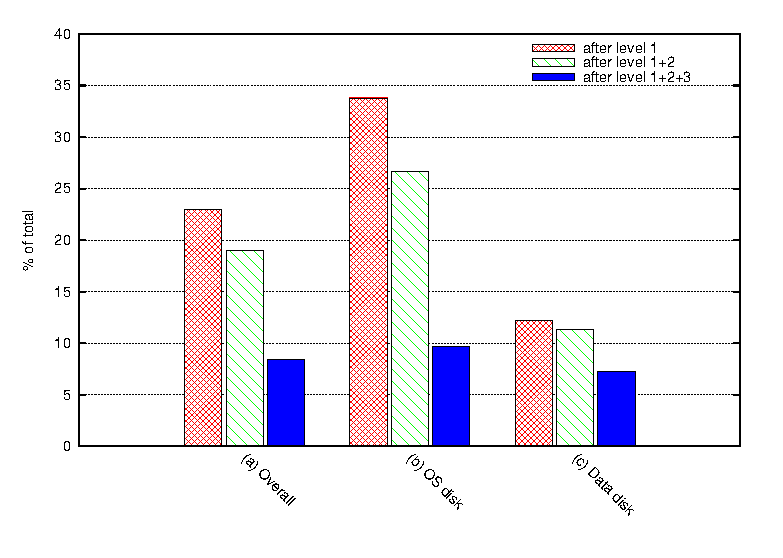
\epsfig{file=images/overall_effect.eps, width=3.5in}
%  \caption{Impacts of 3-level deduplication. The height of each bar is the data size after 
%deduplication divided by the original data size and the unit is percentage. }
%
%  \label{fig:overall}
%\end{figure}



The total local disk usage on
each machine is about 8GB for duplicate detection purpose and most of them for global index. 
Level 1 segment dirty bits identify 78\% of duplicate blocks. For the remaining dirty segments,
block-wise full deduplication removes about additional 74.5\% of duplicates.
The final content copied to the backup storage is reduced by 94.4\% in total.

\begin{figure}
\centering
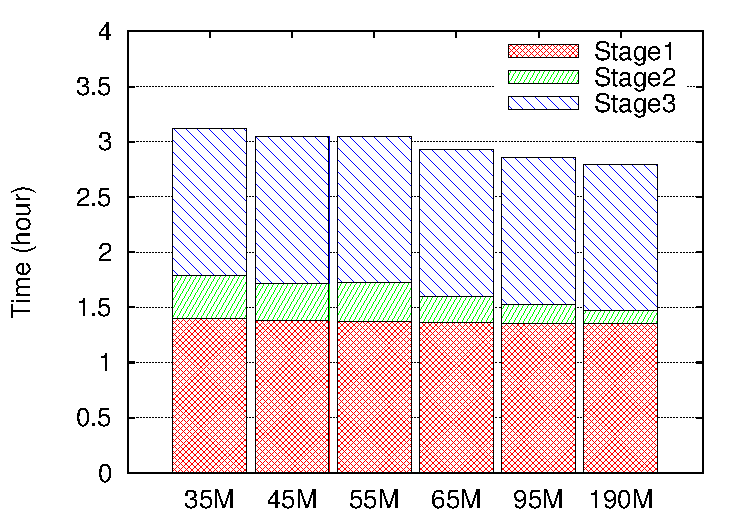
\includegraphics[width=0.4\textwidth]{mem_time.pdf}
\caption{ Parallel time when memory limit varies.}
\label{fig:memory}
\end{figure}

Figure~\ref{fig:memory} shows the total parallel time in hours to backup 2500 VMs on
 a 100-node cluster a  when 
the memory limit $M$ imposed on each node varies  from 20MB to 200MB.
The overall processing time does not have a significant reduction as $M$ increases to 200MB.
The parallel time includes the first scanning time, 
of dirty VM segments to generate block fingerprints, data redistribution for request accumulation,
fingerprint comparison, duplicate summary distribution, and the second scan time for real backup.
The total time is mainly dominated by  the two scans of dirty VM segments.
The time for copying to the final backup storage is overlapped with VM scanning.
%Each scan takes about 1.4 hours.
The aggregated throughput is  about 9.6GB per second,
which is the size of 2500 VM images divided by the parallel time. 
The result shows the backup with multi-stage deduplication  for all VM images can be 
completed in about 2.9 hours with 35MB memory and 8GB disk overhead.
As we vary the cluster size $p$,  the parallel time does  not change much, and  the aggregated throughput
scales up linearly since the number of VMs is  $25p$. 

Table~\ref{tab:overall} shows performance change when memory limit $M$=35MB is imposed and
the number of parititons per machine ($q$) varies from 50 to 1500.
Row 2 is the memory space required to load a partition of global index and detection requests.
When $q=50$, the required memory is 156MB, which  is  not  a viable choice  under  constraint $M=$35MB.  
Row 3 is the parallel time and Row 4 is  the aggregated throughput of  100 nodes.
%The result shows the backup with multi-phase deduplication  for all VM images can be completed in about 3.09 hours
%with the very small resource usage.
Row 5 is  the parallel time if  we use Option 1 with $p\times q$ send buffers 
described in Section~\ref{sect:arch}. 
With the large number of buffers, the available space per buffer reduces significantly as $q$ increases, which leads to
a big increase of IO requests and seek cost.  

\begin{table}[hbt]
\caption{ Performance when the number of partitions per machine node varies and $M$=35MB is imposed.}
\begin{center}
\begin{tabular} {|c|c|c|c|c|c|}
\hline \#Partitions  & 50 & 275  &450 &  750 &  1500 \\
\hline Index+request & 156&  28.4 & 17.4 & 10.7 & 5.2 \\
  (MB)           &  &   &  & &  \\

\hline Total Time  & N/A&  2.9 & 2.91 & 3 & 3.1 \\
  (Hours)           &  &   &  & &  \\
%\hline Throughput/node & N/A&  85MB/s& 90M & 87 & 81 \\
\hline Throughput GB/s& N/A&  9.6& 9.5 & 9.3 & 8.9 \\
\hline Total time & N/A&  7.8& 11.7 & 14.8 & 26 \\
  (Option 1)           &  &   &  & &  \\
\hline
\end{tabular}
\end{center}
\label{tab:overall}
\end{table}

%\begin{verbatim}
%memory
%#partitions/node	50	100	250	275	300	450	500	750	1500	2000
%Memory meta data 0.161	0.0805	0.0322	0.029272727	0.026833333	0.017888889	0.0161	0.010733333	0.005366667	0.004025
%Global index 0.115	0.0575	0.023	0.020909091	0.019166667	0.012777778	0.0115	0.007666667	0.003833333	0.002875
%Seek (Step 1) 0.0212962960.0425 0.106 0.117 0.127777778	0.191666667	0.212962963	0.319444444	0.638888889	0.851851852
%Seek Option 2: 6.388888889	12.77777778	31.94444444	35.13888889	38.33333333	57.5	63.88888889	95.83333333	191.6666667	255.5555556
%Total time 3.059031718	3.078670034	3.131061779	3.137163671	3.141047877	3.313871832	3.296994302	3.377385758	3.689876824	3.901831421
%throughput  per node 0.090805785	0.090226551	0.088716799	0.088544242	0.088434748	0.083822728	0.084251822	0.082246387	0.075281044	0.07119164
%
%\end{verbatim}

%\begin{figure}
%  \centering

%  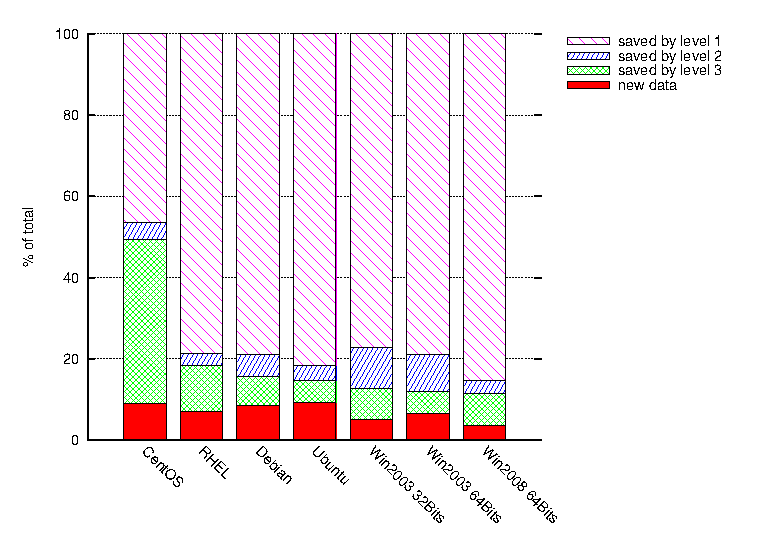
\epsfig{file=images/3level_os.eps, width=3.5in}
%  \caption{Impact of 3-level deduplication for OS releases.}
%  \label{fig:oscds}
%\end{figure}

%To see the impact of multi-level deduplication on different OS releases,
%Some of  OS disks are modified frequently and in some cases,  users even store a large amount of user data on


%\begin{verbatim}
%q= is chosen between 500 or 100
%Memory limit:   20 35M   50M  75M  100M  200M
%req buf	    30M   40M  60   90M     180M
%q:          450     275    275   275 275   
%Time:          3.06  2.9  2.86  2.84 2.834  2.823
%Time for two scans: 2.63  2.63
%\end{verbatim}


%Combining OS disks in all the VMs, we see the overall 7.4TB of data is reduced to 512GB. 
%The extreme binning approach can reduce this data set to 542GB, which is slightly worse. As a reference, 
%perfect deduplication achieves 364GB in this experiment.

%Overall speaking, inner   VM deduplication or  CDS-based deduplication
%can work well alone, but by combining them together we get a fairly good and stable deduplication ratio to 
%all kind of OSes. 
%Compared to a traditional dirty bit approach based on pages of
%each file (e.g. segment in our scheme),
%our CDS-based level 3 approach  can save additional 50\% storage space because many of level 2 block
%content can be eliminated using the CDS also.

\comments{
We have also compared our multi-stage detection approach with an inline approach by combining
dirtybit segment  detection and  the data domain method~\cite{bottleneck08}. 
The bloomer filter setting  results a 1:10 ratio of index reduction for in-memory search before visiting
the disk for the full index with 2\% false positives. The prefetching cache hit ratio is set to be 98.96\% based
a number in ~\cite{bottleneck08}.
We measure its  total time including one scan of VM dirty segments in about 1.38 hours.
That approach takes about 3.19 hours comparable with our scheme while its memory takes
over 1GB with 575MB bloom filters and extra space for prefetching cache. That is an significant amount of space,
competing with other cloud service while memory cost of our setting is  insignificant.
} 
%Our actual cache hit ratio tested is close 90\%.
 %data study, zipf, model of cds size and dedup efficiency
%\section{Results}
In our snapshot deduplication architecture, CDS is the key to achieve greater deduplication than
incremental backup solutions. Our basic assumption of CDS us that VM disks, especially OS disks,
have huge amount of data in common, and such common data can be represented by a relatively smaller data set
because of their high appearence frequency. As a result, the major portion of snapshot deduplication effect shall 
emerge from eliminating the duplication of such a small data set. In this section, we evaluate
the effectiveness of CDS using real user VM disks from our production VM cluster.

\subsection{Experiment Setup}
The data set we use is the same as described in previous section. 
We choose extreme binning and perfect deduplication to compare against.
In all experiments, our deduplication enforces 2MB fix-sized segment boundary, 
and uses TTTD algorithm to divide segment into 4KB variable-sized blocks.
For perfect deduplication and extreme binning, the whole snapshots are splitted
using TTTD with 4KB average size. The original extreme binning paper uses whole file
as the input unit, but that is way too big for our system. 
Thus we split image snapshot files into variable-sized segments base on the block hash list, 
using TTTD with average size of 2MB.

\subsection{OS Disk}
We extract the CDS of OS disks by counting the blocks that will appear in a VM's
block store if no CDS is involved in the deduplication process. The threshold is set to less than
1.5\%, which is quite sufficient to include the OS related data since their duplication is much
heavier than others. Then we use this CDS to run the deduplication process again.
Finally we extracted about 80GB of CDS data from 350 OS disk snapshots,
the corresponding CDS meta occupies 800MB in CDS cache.

\begin{figure}
  \centering
  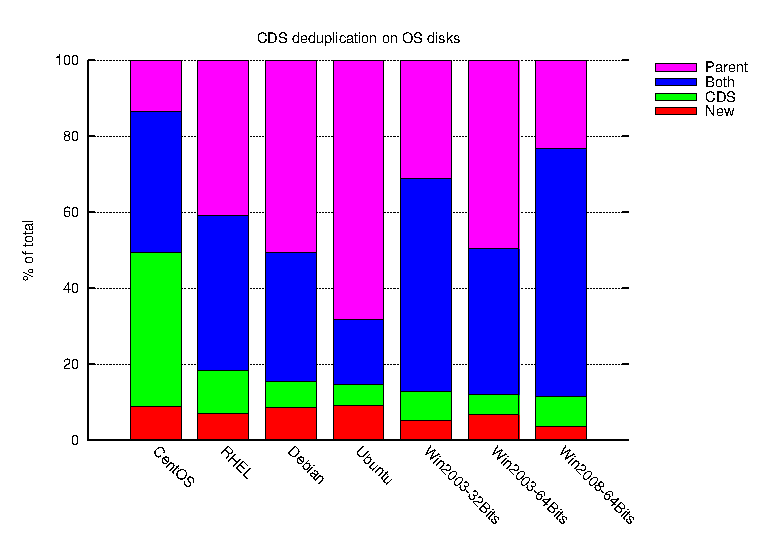
\epsfig{file=images/os_cds_sim.eps, height=2in, width=2.66in}
  \caption{CDS deduplication effect on OS disks}
  \label{fig:oscds}
\end{figure}

For each block, we tag it with one of the following:
\begin{itemize}
\item {New: this block cannot be deduplicated and thus write to block store.}
\item {CDS: this block is deduplicated by CDS.}
\item {Parent: this block is not found in CDS, but is found in parent snapshot's segment recipe.}
\item {Both: this block is both found in CDS and parent snapshot.}
\end{itemize}
As we can see from \ref{fig:oscds}, locality dominates.
This is because the interval between two snapshots is quite short due to our daily snapshot strategy. 
However, locality still doesn't work well on some of the OSes. But CDS, on the contrary,
finds a lot of duplicates that locality can't find, especially in a VM's first snapshot.

Combining all the VMs, we see the overall 7.4TB of data is reduced to 512GB. Extreme bining 
reduces this data set to 542GB, which is slightly worse. As a reference, perfect deduplication achieves
364GB in this experiment.

Overall, none of locality or CDS can solely work well, but by combining them together 
we get fairly good and stable deduplication ratio to all kind of OSes. If compare to all
incremental backup solutions, CDS can save addition 50\%+ of disk space because it greatly reduces
the cross-VM duplicates.

\subsection{Data Disk}
Figure \ref{fig:pd} shows the compression ratio of perfect deduplication at different data scales. 
Basically perfect deduplication would help us save 50\% of space on user data, 
regardless of scale. If we put all these unique data into CDS, we could achieve perfect deduplication, 
which is not affordable. So we need to see how much space saving of perfect 
deduplication can be achieved through a limit size CDS.
\begin{figure}
  \centering
  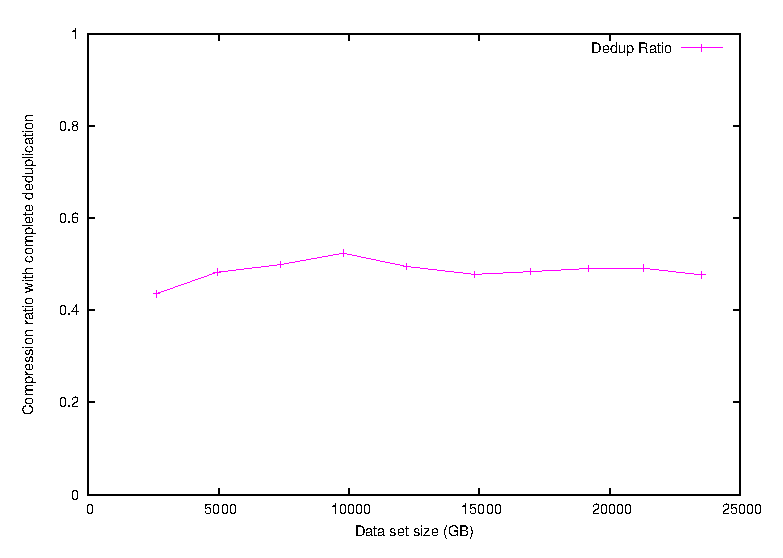
\epsfig{file=images/dedup_ratio.eps, height=2in, width=2.66in}
  \caption{Perfect deduplication on data disks}
  \label{fig:pd}
\end{figure}

We rank unique data blocks by their duplication count, 
and choose the hottest blocks as CDS. 
We define \emph{space saving ratio} as the space saving of CDS divide by 
perfect deduplication saving. Figure \ref{fig:datacdssize} shows the relationship between CDS size and space saving. 
It’s clear a very small amount of CDS data provides more than 50\% saving. 
But this effect decreases when more data are added to CDS. 
The lower bound of CDS space saving ratio is 50\%, which is very easy to accomplish. 

\begin{figure}
  \centering
  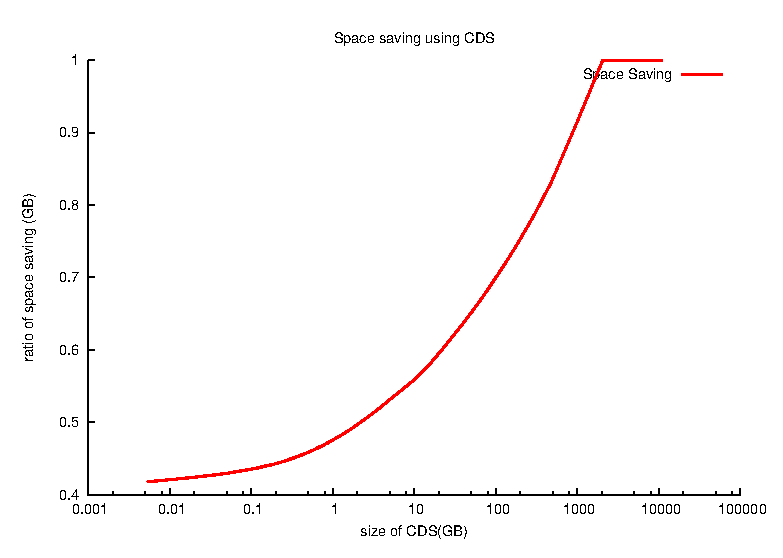
\epsfig{file=images/uniquedata-saving.eps, height=2in, width=2.66in}
  \caption{Size of CDS vesus space saving}
  \label{fig:datacdssize}
\end{figure}

The upper bound of CDS size is restricted by system memory resource.
Figure \ref{fig:datacds} shows how CDS space saving is affected by the system scale. 
In this experiment we first set out a goal of space saving ratio, 
then we watch how much data we need to put into CDS to achieve this goal.
From the graph we can see a 75\% saving goal lead to a stable ratio between 
CDS size and data size, which requires 0.01\% of data to be put in CDS.

Base on above data we can estimate the size of data CDS and its effect. 
Currently we prepared 500MB memory per machine to store CDS meta, then it can represent 50GB of data. 
If we assume each VM has 30GB of user data at runtime, and we host 25 VMs per machine, 
 maintain 10 snapshots per VM, each brings 10\% additional modified data. 
Thus the user data in snapshot system is 1.5TB per machine. So the upper bound of 
$CDS size/ Data size = 0.033$, which is sufficient for the 75\% saving goal.

\begin{figure}
  \centering
  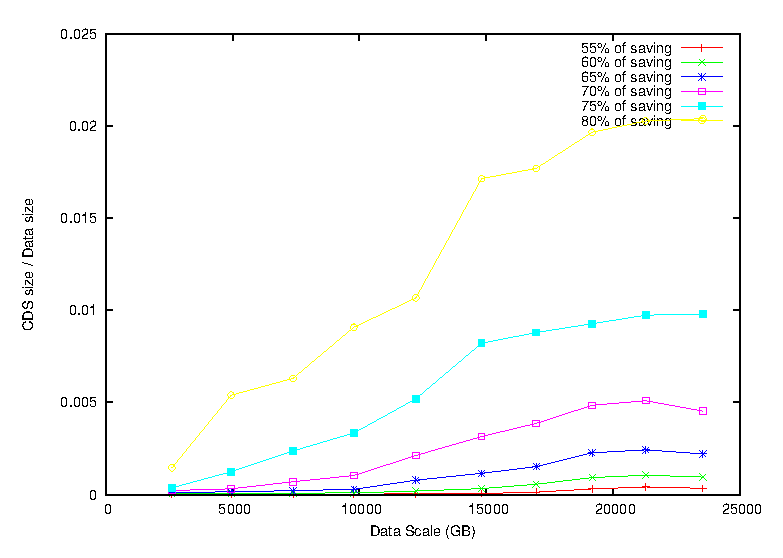
\epsfig{file=images/cds_scale.0.7.eps, height=2in, width=2.66in}
  \caption{CDS deduplication effect on data disks}
  \label{fig:datacds}
\end{figure}

Unlike the CDS of OS disks which is mainly composed of OS related data thus highly predictable, 
data disks is unpredictable because we cannot control what user can put in there. But we still
suspect that highly duplicated data in existing data are very likely to be duplicated again.
So we randomly pick 50 out of 1322 data disks as the new data, and use the rest as existing data
to extract CDS. Using 1.5\% as CDS threshold, we see the total 1198GB of new data is reduced by 
755.8GB, while perfect deduplication can reduce 1017.4GB. So 74.3\% of duplicate blocks are eliminated 
by pre-trained CDS, which is quite satisfiable.

%\section{Related Works}
Several approaches have been previously proposed to enable efficient deduplication in D2D backup.

DDFS\cite{bottleneck08} exploits chunk locality to achieve high-throughput perfect deduplication. 
It preserves locality by a Stream-Informed Segment Layout and exploits locality with Locality Preserved Cache. 
An in-memory Bloom Filter is also used to accelerate non-duplicate chunk identification.

Sparse Indexing\cite{sparseindex09} is an approximate deduplication technique designed for D2D backup. 
It divides data stream into variable-sized multiple kilobytes chunks, and construct multiple megabytes segments
using the same chunking technique, 
which are then sampled and mapped to a compact in-memory sparse index. 
Incoming segments are only deduplicated against several existing similar 
segments selected according to the sparse index.

Both DDFS and Sparse Indexing are designed for D2D backup workloads, 
and do not address the scalability issue in a distributed environment. 
A few scalable deduplication approaches have been proposed recently.

Extreme Binning\cite{extreme_binning09} is a scalable parallel deduplication approach 
that targets at non-traditional backup workloads that consist of low-locality individual files. 
It groups highly similar files into bins, and eliminates duplicate chunks inside each bin. 
Duplicate chunks are allowed to exist among different bins, resulting in approximate deduplication. 
By keeping only the primary index in memory, Extreme Binning can reduce the RAM requirement while 
maintaining a reasonably high throughput. However, their per-file based similarity detection 
is going to group all similar files into one node, which will break load balancing if some files are
huge and similar(e.g., virtual machine images).

MAD2\cite{mad210} is a scalable high-throughput exact duplication approach. 
MAD2 utilizes on-disk Hash Bucket Matrix to preserve fingerprint locality and 
integrates in-memory Dual Cache to capture and exploit locality. 
In addition, MAD2 employs Bloom Filter Array to efficiently identify unique 
incoming fingerprints and indicate where a duplicate may reside. 
By employing a DHT-based Load-Balance technique to distribute file recipes 
and chunk contents among multiple storage nodes in their backup sequences, 
MAD2 further enhances performance with a well balanced load. However, the
data locality does not exist for cloud storage because only changed chunks are expected
to be uploaded, and
the heavy usage of memory and CPU indicates such exact deduplication backup systems
need storage-exclusive servers with hardware replication support, which is not a general case 
for the cloud..

HYDRAstor\cite{hydrastor09}, a scalable secondary storage solution, 
constructs its backend using a grid of storage nodes built around a distributed hash table. 
The backend maintains large-scale variable-sized, content-addressed, immutable, 
and highly-resilient data blocks that are logically organized in a directed acyclic graph. 
Duplicate chunks are eliminated according to their hashes. 
HYDRAstor adopts an average chunk size of 64KB, among other constraints, 
to keep all the metadata in memory and avoid the duplicate-lookup disk bottleneck. 
This degrades the space efficiency of deduplication, and still requires huge amount of memory.

We believe a deduplication backend of cloud storage must have scalability and
 high availability built in mind, being able to run on low-cost non-proprietary machines.
  Unlike sloud, all above systems lack one or a few such properties. All exact deduplication approaches
are too costly, this is why we choose similarity based approach to trade deduplication
accuracy for speed. 

Eariler deduplication systems mainly focus on improving storage space efficiency by eliminating 
duplicates at the file level, fixed-size block level, or variable-sized chunk level. 
EMC's Centera\cite{emc_centera} identify and eliminate duplicate data by comparing 
the hash of the whole file or fixed content. Venti\cite{venti02}, a block-level archival storage, 
removes redundant fixed-size data blocks by comparing their secure hashes. Pastiche\cite{pastiche02} 
utilizes chunk-level duplicate detection to construct a resource-saving peer-to-peer backup network. 
Deep Store\cite{deepstore05}, a large scale archival storage system, uses both variable-sized 
chunk-level deduplication and delta compression to save storage. Jumbo Store\cite{jumbo07} organizes 
variable-sized chunks into Hash-Based Directed Acyclic Graphs to save both storage and 
bandwidth while performing incremental upload and versioning for a utility rendering service. 

Duplicate detection technique has also been used in bandwidth-saving synchronization protocols\cite{rsync} 
and low-bandwidth network file systems\cite{lbfs01}.
%\input{future}
\section{Conclusion Remarks}
\label{sect:final}

The contribution  of this work is a low-cost multi-stage parallel deduplication solution.
Because of separation  of duplicate detection and actual backup,
we are able to evenly distribute  fingerprint comparison among clustered machine
nodes, and only load one partition at time at each machine for in-memory comparison.
The tradeoff is that every machine has to read dirty segments twice 
and that some deduplication requests are delayed for staged processing.  

The evaluation shows that the overall 
deduplication time and throughput of 100 machines  are satisfactory with 
about 9.6GB per second for 2500 VMs. During processing, each machine uses 
only  35MB memory, 8GB disk space, and an upto 10\% of one CPU core with a single thread  execution.
Thus the proposed  scheme does not take a significant  amount of the resource away
to compete with the existing cloud services.
%While using an insignificant system resource,
%When the cluster size changes, our experiment also shows a linear speedup of overall throughputs
%because highly parallel fingerprint comparisons.  
%The cluster  of 100 nodes and 2500 VMs can deliver about 
%8.8GB per second deduplication performance.  We expect the system performs well in a larger cloud 
%setting and 
Our future work is to conduct more investigations with production workloads.
%We currently assume each machine performs backup for all VMs hosted and in practice, the system only
%needs to backup active VMs and thus the overall backup time would actually be much smaller.

%in parallel among all machines and  each machine full duplication detection is 
%Another optimization is to allocate and control
%buffer space for exchanging  detection messages and duplicate summary among machines.
%snapshot service in VM cloud. 
%Inner-VM deduplication localizes backup data dependency and exposes more parallelism  
%while cross-VM deduplication with a small common data set
%effectively  covers a large amount of duplicated data.
%Our solution accomplishes the majority of
%potential global deduplication saving while still meets stringent cloud resources requirement. 
%Evaluation using real user's VM data shows
%our solution can accomplish 75\% of what complete global
%deduplication can do. 
%Compare to today's widely-used snapshot technique, our scheme reduces almost
%two-third of snapshot storage cost.
%Finally, our scheme uses a very small amount of memory on each node, and leaves
%room for additional optimization we are further studying.


%The memory requirement and disk usage for the proposed solution is very small while the overall thoughput
%and backup process timing is not compromised. 
%Our experiments show that  the proposed scheme 
%uses a very small amount of system resources while accomplishing a satisfactory backup throughput
%in a large cloud setting.
%which only reqiires a very small amount of memory and CPU resource.  
%Experimental results  show the proposed scheme  can achieve high deduplication ratio while using
%a  small  amount of cloud resources. 

%Our system compares well with Amazon Glacier, in that, both of them are low-cost archival systems, 
%supporting lazy storage with asynchronous notification mechanisms and achieve parallelism by 
%reading/writing from multiple storage nodes/disks simultaneously. At the same time, 


%While dirtybit-based technique can identify unmodified data between versions, 
%full deduplication with fingerprint comparison  can remove more redundant content
%at the cost of computing resources.
%with  for similarity comparison and   reliability handling.
%Current snapshot deduplication is mainly done through copy-on-write 
%on fixed-size disk blocks. Such solutions cannot handle the
% cross VM data duplication because VMs do not share any data. 
%In addition, storing VM images and their snapshots
%in the same storage engine reduce the underline design flexibility because 
%these two kinds of data have distinct access requirements.
%In this paper, 
%we show that there is a large amount of duplicated data shared amongy virtual machines
%through a production VM data study and thus it is expective to perform cross-machine deduplication. 
% first perform a large scale study in production VM clusters 
%to show that cross VM data duplication is severe due to they have large amount of
%common data. Then our data analysis finds out that the overall data duplication pattern follows the Zipf's law.
%Base on these discoveries, we propose a snapshot storage deduplication scheme using variable-size chunking
%to address the above problem efficiently.
%We eliminate the majority of cross VM data duplication by pre-select
%a small set of frequently seen data blocks to be shared globally, and we also remove
%many cross snapshot duplication by using smaller chunking granuarity and locality.




%\section*{Acknowledgments}
%{
%We would like to thank Weicai Chen and Shikun Tian from Alibaba for their kind support, 
%and the anonymous referees for their comments.
%Wei Zhang has received internship support from Alibaba  for VM backup system development.
%This work was supported in part by NSF IIS-1118106.
%Any opinions, findings, and conclusions or recommendations expressed in this material are those of the authors and
%do not necessarily reflect the views of Alibaba or the National Science Foundation.
%}
%Noted that 6\% is still significant, which is about 24GB per each VM and for a 1000 node Aliyun cluster,
%this is about 600 terabytes.
 
%Our experiments show th
%our solution can eliminate the majority of data duplication with a tiny fraction of
%block hash index store in memory. It does not only saves valuable system resouces in
%the VM cloud, but also makes deduplication much faster.
%
%
%Using  50 user VM data out of 1322 data disks as the training data and
%with  1.5\% as CDS threshold, we see the total 1198GB of new data is reduced by
%755.8GB, while perfect deduplication can reduce 1017.4GB. So 74.3\% of duplicate blocks are eliminated
%by pre-trained CDS, which is quite satisfactory.




{\bf Acknowledgment.} We thank Hong Tong for his help and support.
%Renu Tewari, and anonymous referees in for their valuable comments.
This work is supported in part by NSF IIS-1118106. 
Any opinions, findings, conclusions or recommendations expressed in this material
are those of the authors and
do not necessarily reflect the views of the National Science Foundation.


      %\setlength{\itemsep}{ex}%
%      \setlength{\parskip}{0ex}%
%\setlength{\itemsep}{-3mm}

	%\linespread{0.3} 
%  \let\oldthebibliography=\thebibliography
%  \let\endoldthebibliography=\endthebibliography
%  \renewenvironment{thebibliography}[1]{%
%    \begin{oldthebibliography}{#1}%
%      \setlength{\parskip}{-0.02ex}%
%      \setlength{\itemsep}{-0.02ex}%
%      \setlength{\baselineskip}{-0.02ex}%

%  }%
%  {%
%    \end{oldthebibliography}%
%  }
{\small
\bibliographystyle{abbrv}
\bibliography{library,dedup1}
}
\end{document}
